\documentclass[twoside]{book}

% Packages required by doxygen
\usepackage{fixltx2e}
\usepackage{calc}
\usepackage{doxygen}
\usepackage[export]{adjustbox} % also loads graphicx
\usepackage{graphicx}
\usepackage[utf8]{inputenc}
\usepackage{makeidx}
\usepackage{multicol}
\usepackage{multirow}
\PassOptionsToPackage{warn}{textcomp}
\usepackage{textcomp}
\usepackage[nointegrals]{wasysym}
\usepackage[table]{xcolor}

% Font selection
\usepackage[T1]{fontenc}
\usepackage[scaled=.90]{helvet}
\usepackage{courier}
\usepackage{amssymb}
\usepackage{sectsty}
\renewcommand{\familydefault}{\sfdefault}
\allsectionsfont{%
  \fontseries{bc}\selectfont%
  \color{darkgray}%
}
\renewcommand{\DoxyLabelFont}{%
  \fontseries{bc}\selectfont%
  \color{darkgray}%
}
\newcommand{\+}{\discretionary{\mbox{\scriptsize$\hookleftarrow$}}{}{}}

% Page & text layout
\usepackage{geometry}
\geometry{%
  a4paper,%
  top=2.5cm,%
  bottom=2.5cm,%
  left=2.5cm,%
  right=2.5cm%
}
\tolerance=750
\hfuzz=15pt
\hbadness=750
\setlength{\emergencystretch}{15pt}
\setlength{\parindent}{0cm}
\setlength{\parskip}{3ex plus 2ex minus 2ex}
\makeatletter
\renewcommand{\paragraph}{%
  \@startsection{paragraph}{4}{0ex}{-1.0ex}{1.0ex}{%
    \normalfont\normalsize\bfseries\SS@parafont%
  }%
}
\renewcommand{\subparagraph}{%
  \@startsection{subparagraph}{5}{0ex}{-1.0ex}{1.0ex}{%
    \normalfont\normalsize\bfseries\SS@subparafont%
  }%
}
\makeatother

% Headers & footers
\usepackage{fancyhdr}
\pagestyle{fancyplain}
\fancyhead[LE]{\fancyplain{}{\bfseries\thepage}}
\fancyhead[CE]{\fancyplain{}{}}
\fancyhead[RE]{\fancyplain{}{\bfseries\leftmark}}
\fancyhead[LO]{\fancyplain{}{\bfseries\rightmark}}
\fancyhead[CO]{\fancyplain{}{}}
\fancyhead[RO]{\fancyplain{}{\bfseries\thepage}}
\fancyfoot[LE]{\fancyplain{}{}}
\fancyfoot[CE]{\fancyplain{}{}}
\fancyfoot[RE]{\fancyplain{}{\bfseries\scriptsize Generated by Doxygen }}
\fancyfoot[LO]{\fancyplain{}{\bfseries\scriptsize Generated by Doxygen }}
\fancyfoot[CO]{\fancyplain{}{}}
\fancyfoot[RO]{\fancyplain{}{}}
\renewcommand{\footrulewidth}{0.4pt}
\renewcommand{\chaptermark}[1]{%
  \markboth{#1}{}%
}
\renewcommand{\sectionmark}[1]{%
  \markright{\thesection\ #1}%
}

% Indices & bibliography
\usepackage{natbib}
\usepackage[titles]{tocloft}
\setcounter{tocdepth}{3}
\setcounter{secnumdepth}{5}
\makeindex

% Hyperlinks (required, but should be loaded last)
\usepackage{ifpdf}
\ifpdf
  \usepackage[pdftex,pagebackref=true]{hyperref}
\else
  \usepackage[ps2pdf,pagebackref=true]{hyperref}
\fi
\hypersetup{%
  colorlinks=true,%
  linkcolor=blue,%
  citecolor=blue,%
  unicode%
}

% Custom commands
\newcommand{\clearemptydoublepage}{%
  \newpage{\pagestyle{empty}\cleardoublepage}%
}

\usepackage{caption}
\captionsetup{labelsep=space,justification=centering,font={bf},singlelinecheck=off,skip=4pt,position=top}

%===== C O N T E N T S =====

\begin{document}

% Titlepage & ToC
\hypersetup{pageanchor=false,
             bookmarksnumbered=true,
             pdfencoding=unicode
            }
\pagenumbering{alph}
\begin{titlepage}
\vspace*{7cm}
\begin{center}%
{\Large R\+PA }\\
\vspace*{1cm}
{\large Generated by Doxygen 1.8.14}\\
\end{center}
\end{titlepage}
\clearemptydoublepage
\pagenumbering{roman}
\tableofcontents
\clearemptydoublepage
\pagenumbering{arabic}
\hypersetup{pageanchor=true}

%--- Begin generated contents ---
\chapter{Class Index}
\section{Class List}
Here are the classes, structs, unions and interfaces with brief descriptions\+:\begin{DoxyCompactList}
\item\contentsline{section}{\mbox{\hyperlink{class_array___sequences}{Array\+\_\+\+Sequences}} }{\pageref{class_array___sequences}}{}
\item\contentsline{section}{\mbox{\hyperlink{class_optimization___toolbox}{Optimization\+\_\+\+Toolbox}} }{\pageref{class_optimization___toolbox}}{}
\item\contentsline{section}{\mbox{\hyperlink{class_p_c_r___profile}{P\+C\+R\+\_\+\+Profile}} }{\pageref{class_p_c_r___profile}}{}
\item\contentsline{section}{\mbox{\hyperlink{class_p_c_r___profile___array}{P\+C\+R\+\_\+\+Profile\+\_\+\+Array}} }{\pageref{class_p_c_r___profile___array}}{}
\item\contentsline{section}{\mbox{\hyperlink{class_primer___set}{Primer\+\_\+\+Set}} }{\pageref{class_primer___set}}{}
\item\contentsline{section}{\mbox{\hyperlink{class_sequence}{Sequence}} }{\pageref{class_sequence}}{}
\item\contentsline{section}{\mbox{\hyperlink{struct_sortable___pareto}{Sortable\+\_\+\+Pareto}} }{\pageref{struct_sortable___pareto}}{}
\end{DoxyCompactList}

\chapter{Class Documentation}
\hypertarget{class_array___sequences}{}\section{Array\+\_\+\+Sequences Class Reference}
\label{class_array___sequences}\index{Array\+\_\+\+Sequences@{Array\+\_\+\+Sequences}}


{\ttfamily \#include $<$Array\+\_\+\+Sequences.\+h$>$}

\subsection*{Public Member Functions}
\begin{DoxyCompactItemize}
\item 
\mbox{\hyperlink{class_array___sequences_a4960de248d6dceefcae88e66a5a51e8b}{Array\+\_\+\+Sequences}} (char $\ast$filename, unsigned int primer\+\_\+value=0, ostream \&err\+\_\+msg=cout)
\item 
\mbox{\hyperlink{class_array___sequences_ac33a3e2bdca116464baa042a2aea2518}{Array\+\_\+\+Sequences}} (ostream \&err\+\_\+msg=cout)
\item 
\mbox{\hyperlink{class_array___sequences_a740bb50d572c522a093f52a1c5c79e03}{$\sim$\+Array\+\_\+\+Sequences}} ()
\item 
bool \mbox{\hyperlink{class_array___sequences_ab0735daa57cd712e08843e9c79e40488}{show\+\_\+\+Statistics}} (ostream \&out=cout, ostream \&err\+\_\+msg=cout)
\item 
bool \mbox{\hyperlink{class_array___sequences_ad197ef5c061d0cfc564afe5504fa4961}{show\+\_\+\+All}} (ostream \&out=cout, ostream \&err\+\_\+msg=cout)
\item 
bool \mbox{\hyperlink{class_array___sequences_ae4e47e71792255275b01afd35456a9a0}{add\+\_\+sequence}} (\mbox{\hyperlink{class_sequence}{Sequence}} $\ast$\+\_\+sequence, unsigned int primer\+\_\+value=0, ostream \&err\+\_\+msg=cout)
\item 
bool \mbox{\hyperlink{class_array___sequences_aa5e6c65a85deac945f5d11442c4eb319}{add\+\_\+sequence}} (char $\ast$\+\_\+sequence, unsigned int \+\_\+sequence\+\_\+length, unsigned int primer\+\_\+value=0, ostream \&err\+\_\+msg=cout)
\item 
unsigned int \mbox{\hyperlink{class_array___sequences_a76fd0aa59aaf720c64088ab9c900668f}{get\+\_\+number\+\_\+of\+\_\+sequences}} ()
\item 
\mbox{\hyperlink{class_sequence}{Sequence}} $\ast$ \mbox{\hyperlink{class_array___sequences_a029592cf35f56df0714e5326a3901b74}{get\+\_\+pointer\+\_\+to\+\_\+sequence\+\_\+object}} (unsigned int position)
\end{DoxyCompactItemize}
\subsection*{Static Public Attributes}
\begin{DoxyCompactItemize}
\item 
static unsigned int \mbox{\hyperlink{class_array___sequences_a05103713b20762f7e2a4a970a35514f2}{max\+\_\+sequence\+\_\+length}} = 1000000000
\item 
static unsigned int \mbox{\hyperlink{class_array___sequences_a15164d8882eac2d8cf368f74fde967d2}{max\+\_\+number\+\_\+of\+\_\+sequences}} = 5000
\end{DoxyCompactItemize}


\subsection{Detailed Description}


Definition at line 16 of file Array\+\_\+\+Sequences.\+h.



\subsection{Constructor \& Destructor Documentation}
\mbox{\Hypertarget{class_array___sequences_a4960de248d6dceefcae88e66a5a51e8b}\label{class_array___sequences_a4960de248d6dceefcae88e66a5a51e8b}} 
\index{Array\+\_\+\+Sequences@{Array\+\_\+\+Sequences}!Array\+\_\+\+Sequences@{Array\+\_\+\+Sequences}}
\index{Array\+\_\+\+Sequences@{Array\+\_\+\+Sequences}!Array\+\_\+\+Sequences@{Array\+\_\+\+Sequences}}
\subsubsection{\texorpdfstring{Array\+\_\+\+Sequences()}{Array\_Sequences()}\hspace{0.1cm}{\footnotesize\ttfamily [1/2]}}
{\footnotesize\ttfamily Array\+\_\+\+Sequences\+::\+Array\+\_\+\+Sequences (\begin{DoxyParamCaption}\item[{char $\ast$}]{filename,  }\item[{unsigned int}]{primer\+\_\+value = {\ttfamily 0},  }\item[{ostream \&}]{err\+\_\+msg = {\ttfamily cout} }\end{DoxyParamCaption})}



Definition at line 60 of file Array\+\_\+\+Sequences.\+h.

\mbox{\Hypertarget{class_array___sequences_ac33a3e2bdca116464baa042a2aea2518}\label{class_array___sequences_ac33a3e2bdca116464baa042a2aea2518}} 
\index{Array\+\_\+\+Sequences@{Array\+\_\+\+Sequences}!Array\+\_\+\+Sequences@{Array\+\_\+\+Sequences}}
\index{Array\+\_\+\+Sequences@{Array\+\_\+\+Sequences}!Array\+\_\+\+Sequences@{Array\+\_\+\+Sequences}}
\subsubsection{\texorpdfstring{Array\+\_\+\+Sequences()}{Array\_Sequences()}\hspace{0.1cm}{\footnotesize\ttfamily [2/2]}}
{\footnotesize\ttfamily Array\+\_\+\+Sequences\+::\+Array\+\_\+\+Sequences (\begin{DoxyParamCaption}\item[{ostream \&}]{err\+\_\+msg = {\ttfamily cout} }\end{DoxyParamCaption})}



Definition at line 53 of file Array\+\_\+\+Sequences.\+h.

\mbox{\Hypertarget{class_array___sequences_a740bb50d572c522a093f52a1c5c79e03}\label{class_array___sequences_a740bb50d572c522a093f52a1c5c79e03}} 
\index{Array\+\_\+\+Sequences@{Array\+\_\+\+Sequences}!````~Array\+\_\+\+Sequences@{$\sim$\+Array\+\_\+\+Sequences}}
\index{````~Array\+\_\+\+Sequences@{$\sim$\+Array\+\_\+\+Sequences}!Array\+\_\+\+Sequences@{Array\+\_\+\+Sequences}}
\subsubsection{\texorpdfstring{$\sim$\+Array\+\_\+\+Sequences()}{~Array\_Sequences()}}
{\footnotesize\ttfamily Array\+\_\+\+Sequences\+::$\sim$\+Array\+\_\+\+Sequences (\begin{DoxyParamCaption}{ }\end{DoxyParamCaption})}



Definition at line 45 of file Array\+\_\+\+Sequences.\+h.



\subsection{Member Function Documentation}
\mbox{\Hypertarget{class_array___sequences_ae4e47e71792255275b01afd35456a9a0}\label{class_array___sequences_ae4e47e71792255275b01afd35456a9a0}} 
\index{Array\+\_\+\+Sequences@{Array\+\_\+\+Sequences}!add\+\_\+sequence@{add\+\_\+sequence}}
\index{add\+\_\+sequence@{add\+\_\+sequence}!Array\+\_\+\+Sequences@{Array\+\_\+\+Sequences}}
\subsubsection{\texorpdfstring{add\+\_\+sequence()}{add\_sequence()}\hspace{0.1cm}{\footnotesize\ttfamily [1/2]}}
{\footnotesize\ttfamily bool Array\+\_\+\+Sequences\+::add\+\_\+sequence (\begin{DoxyParamCaption}\item[{\mbox{\hyperlink{class_sequence}{Sequence}} $\ast$}]{\+\_\+sequence,  }\item[{unsigned int}]{primer\+\_\+value = {\ttfamily 0},  }\item[{ostream \&}]{err\+\_\+msg = {\ttfamily cout} }\end{DoxyParamCaption})}



Definition at line 141 of file Array\+\_\+\+Sequences.\+h.

Here is the call graph for this function\+:
\nopagebreak
\begin{figure}[H]
\begin{center}
\leavevmode
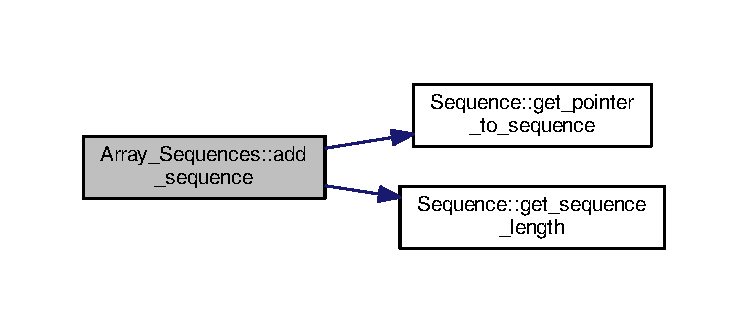
\includegraphics[width=350pt]{class_array___sequences_ae4e47e71792255275b01afd35456a9a0_cgraph}
\end{center}
\end{figure}
\mbox{\Hypertarget{class_array___sequences_aa5e6c65a85deac945f5d11442c4eb319}\label{class_array___sequences_aa5e6c65a85deac945f5d11442c4eb319}} 
\index{Array\+\_\+\+Sequences@{Array\+\_\+\+Sequences}!add\+\_\+sequence@{add\+\_\+sequence}}
\index{add\+\_\+sequence@{add\+\_\+sequence}!Array\+\_\+\+Sequences@{Array\+\_\+\+Sequences}}
\subsubsection{\texorpdfstring{add\+\_\+sequence()}{add\_sequence()}\hspace{0.1cm}{\footnotesize\ttfamily [2/2]}}
{\footnotesize\ttfamily bool Array\+\_\+\+Sequences\+::add\+\_\+sequence (\begin{DoxyParamCaption}\item[{char $\ast$}]{\+\_\+sequence,  }\item[{unsigned int}]{\+\_\+sequence\+\_\+length,  }\item[{unsigned int}]{primer\+\_\+value = {\ttfamily 0},  }\item[{ostream \&}]{err\+\_\+msg = {\ttfamily cout} }\end{DoxyParamCaption})}



Definition at line 128 of file Array\+\_\+\+Sequences.\+h.

\mbox{\Hypertarget{class_array___sequences_a76fd0aa59aaf720c64088ab9c900668f}\label{class_array___sequences_a76fd0aa59aaf720c64088ab9c900668f}} 
\index{Array\+\_\+\+Sequences@{Array\+\_\+\+Sequences}!get\+\_\+number\+\_\+of\+\_\+sequences@{get\+\_\+number\+\_\+of\+\_\+sequences}}
\index{get\+\_\+number\+\_\+of\+\_\+sequences@{get\+\_\+number\+\_\+of\+\_\+sequences}!Array\+\_\+\+Sequences@{Array\+\_\+\+Sequences}}
\subsubsection{\texorpdfstring{get\+\_\+number\+\_\+of\+\_\+sequences()}{get\_number\_of\_sequences()}}
{\footnotesize\ttfamily unsigned int Array\+\_\+\+Sequences\+::get\+\_\+number\+\_\+of\+\_\+sequences (\begin{DoxyParamCaption}{ }\end{DoxyParamCaption})\hspace{0.3cm}{\ttfamily [inline]}}



Definition at line 38 of file Array\+\_\+\+Sequences.\+h.

Here is the caller graph for this function\+:
\nopagebreak
\begin{figure}[H]
\begin{center}
\leavevmode
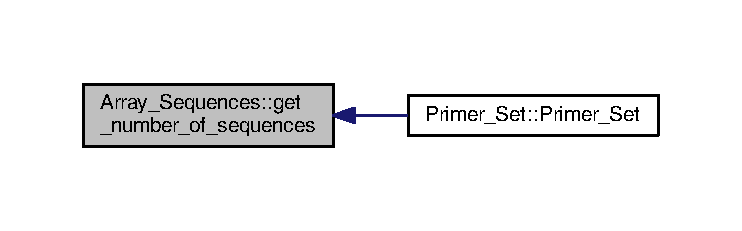
\includegraphics[width=350pt]{class_array___sequences_a76fd0aa59aaf720c64088ab9c900668f_icgraph}
\end{center}
\end{figure}
\mbox{\Hypertarget{class_array___sequences_a029592cf35f56df0714e5326a3901b74}\label{class_array___sequences_a029592cf35f56df0714e5326a3901b74}} 
\index{Array\+\_\+\+Sequences@{Array\+\_\+\+Sequences}!get\+\_\+pointer\+\_\+to\+\_\+sequence\+\_\+object@{get\+\_\+pointer\+\_\+to\+\_\+sequence\+\_\+object}}
\index{get\+\_\+pointer\+\_\+to\+\_\+sequence\+\_\+object@{get\+\_\+pointer\+\_\+to\+\_\+sequence\+\_\+object}!Array\+\_\+\+Sequences@{Array\+\_\+\+Sequences}}
\subsubsection{\texorpdfstring{get\+\_\+pointer\+\_\+to\+\_\+sequence\+\_\+object()}{get\_pointer\_to\_sequence\_object()}}
{\footnotesize\ttfamily \mbox{\hyperlink{class_sequence}{Sequence}}$\ast$ Array\+\_\+\+Sequences\+::get\+\_\+pointer\+\_\+to\+\_\+sequence\+\_\+object (\begin{DoxyParamCaption}\item[{unsigned int}]{position }\end{DoxyParamCaption})\hspace{0.3cm}{\ttfamily [inline]}}



Definition at line 39 of file Array\+\_\+\+Sequences.\+h.

Here is the caller graph for this function\+:
\nopagebreak
\begin{figure}[H]
\begin{center}
\leavevmode
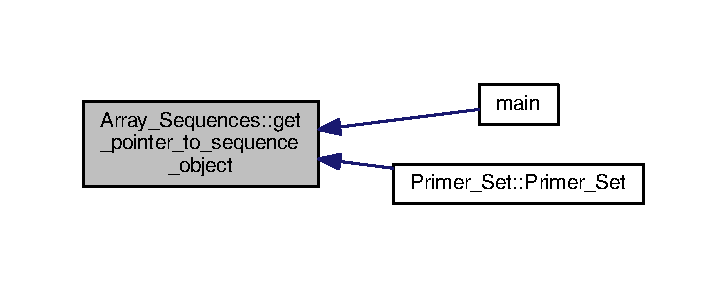
\includegraphics[width=349pt]{class_array___sequences_a029592cf35f56df0714e5326a3901b74_icgraph}
\end{center}
\end{figure}
\mbox{\Hypertarget{class_array___sequences_ad197ef5c061d0cfc564afe5504fa4961}\label{class_array___sequences_ad197ef5c061d0cfc564afe5504fa4961}} 
\index{Array\+\_\+\+Sequences@{Array\+\_\+\+Sequences}!show\+\_\+\+All@{show\+\_\+\+All}}
\index{show\+\_\+\+All@{show\+\_\+\+All}!Array\+\_\+\+Sequences@{Array\+\_\+\+Sequences}}
\subsubsection{\texorpdfstring{show\+\_\+\+All()}{show\_All()}}
{\footnotesize\ttfamily bool Array\+\_\+\+Sequences\+::show\+\_\+\+All (\begin{DoxyParamCaption}\item[{ostream \&}]{out = {\ttfamily cout},  }\item[{ostream \&}]{err\+\_\+msg = {\ttfamily cout} }\end{DoxyParamCaption})}



Definition at line 154 of file Array\+\_\+\+Sequences.\+h.

\mbox{\Hypertarget{class_array___sequences_ab0735daa57cd712e08843e9c79e40488}\label{class_array___sequences_ab0735daa57cd712e08843e9c79e40488}} 
\index{Array\+\_\+\+Sequences@{Array\+\_\+\+Sequences}!show\+\_\+\+Statistics@{show\+\_\+\+Statistics}}
\index{show\+\_\+\+Statistics@{show\+\_\+\+Statistics}!Array\+\_\+\+Sequences@{Array\+\_\+\+Sequences}}
\subsubsection{\texorpdfstring{show\+\_\+\+Statistics()}{show\_Statistics()}}
{\footnotesize\ttfamily bool Array\+\_\+\+Sequences\+::show\+\_\+\+Statistics (\begin{DoxyParamCaption}\item[{ostream \&}]{out = {\ttfamily cout},  }\item[{ostream \&}]{err\+\_\+msg = {\ttfamily cout} }\end{DoxyParamCaption})}



Definition at line 146 of file Array\+\_\+\+Sequences.\+h.

Here is the caller graph for this function\+:
\nopagebreak
\begin{figure}[H]
\begin{center}
\leavevmode
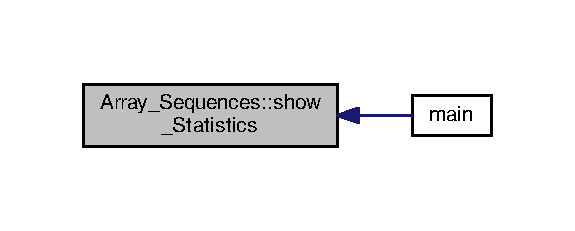
\includegraphics[width=276pt]{class_array___sequences_ab0735daa57cd712e08843e9c79e40488_icgraph}
\end{center}
\end{figure}


\subsection{Member Data Documentation}
\mbox{\Hypertarget{class_array___sequences_a15164d8882eac2d8cf368f74fde967d2}\label{class_array___sequences_a15164d8882eac2d8cf368f74fde967d2}} 
\index{Array\+\_\+\+Sequences@{Array\+\_\+\+Sequences}!max\+\_\+number\+\_\+of\+\_\+sequences@{max\+\_\+number\+\_\+of\+\_\+sequences}}
\index{max\+\_\+number\+\_\+of\+\_\+sequences@{max\+\_\+number\+\_\+of\+\_\+sequences}!Array\+\_\+\+Sequences@{Array\+\_\+\+Sequences}}
\subsubsection{\texorpdfstring{max\+\_\+number\+\_\+of\+\_\+sequences}{max\_number\_of\_sequences}}
{\footnotesize\ttfamily unsigned int Array\+\_\+\+Sequences\+::max\+\_\+number\+\_\+of\+\_\+sequences = 5000\hspace{0.3cm}{\ttfamily [static]}}



Definition at line 24 of file Array\+\_\+\+Sequences.\+h.

\mbox{\Hypertarget{class_array___sequences_a05103713b20762f7e2a4a970a35514f2}\label{class_array___sequences_a05103713b20762f7e2a4a970a35514f2}} 
\index{Array\+\_\+\+Sequences@{Array\+\_\+\+Sequences}!max\+\_\+sequence\+\_\+length@{max\+\_\+sequence\+\_\+length}}
\index{max\+\_\+sequence\+\_\+length@{max\+\_\+sequence\+\_\+length}!Array\+\_\+\+Sequences@{Array\+\_\+\+Sequences}}
\subsubsection{\texorpdfstring{max\+\_\+sequence\+\_\+length}{max\_sequence\_length}}
{\footnotesize\ttfamily unsigned int Array\+\_\+\+Sequences\+::max\+\_\+sequence\+\_\+length = 1000000000\hspace{0.3cm}{\ttfamily [static]}}



Definition at line 23 of file Array\+\_\+\+Sequences.\+h.



The documentation for this class was generated from the following file\+:\begin{DoxyCompactItemize}
\item 
R\+P\+A/\mbox{\hyperlink{_array___sequences_8h}{Array\+\_\+\+Sequences.\+h}}\end{DoxyCompactItemize}

\hypertarget{class_optimization___toolbox}{}\section{Optimization\+\_\+\+Toolbox Class Reference}
\label{class_optimization___toolbox}\index{Optimization\+\_\+\+Toolbox@{Optimization\+\_\+\+Toolbox}}
\subsection*{Static Public Member Functions}
\begin{DoxyCompactItemize}
\item 
\mbox{\Hypertarget{class_optimization___toolbox_acb0793203243d200d9154f2e98011d44}\label{class_optimization___toolbox_acb0793203243d200d9154f2e98011d44}} 
static bool {\bfseries calculate\+\_\+pareto\+\_\+frontier} (double $\ast$x, double $\ast$y, bool $\ast$paretto\+\_\+set, unsigned int number\+\_\+of\+\_\+values, bool maximize\+\_\+x, bool maximize\+\_\+y, ostream \&err\+\_\+msg=cout)
\item 
\mbox{\Hypertarget{class_optimization___toolbox_a44f2c18904985dd9591efe0a63bfae9b}\label{class_optimization___toolbox_a44f2c18904985dd9591efe0a63bfae9b}} 
static bool {\bfseries convert\+\_\+primer\+\_\+txt\+\_\+to\+\_\+int} (char $\ast$\+\_\+primer, unsigned int primer\+\_\+length, unsigned int \&primer\+\_\+value, ostream \&err\+\_\+msg=cout)
\end{DoxyCompactItemize}


The documentation for this class was generated from the following file\+:\begin{DoxyCompactItemize}
\item 
C\+:/\+Users/\+Kamil/\+Documents/\+R\+P\+A-\/\+Optimization/\+R\+P\+A/Optimization\+\_\+\+Toolbox.\+h\end{DoxyCompactItemize}

\hypertarget{class_p_c_r___profile}{}\section{P\+C\+R\+\_\+\+Profile Class Reference}
\label{class_p_c_r___profile}\index{P\+C\+R\+\_\+\+Profile@{P\+C\+R\+\_\+\+Profile}}


{\ttfamily \#include $<$P\+C\+R\+\_\+\+Profile.\+h$>$}

\subsection*{Public Member Functions}
\begin{DoxyCompactItemize}
\item 
\mbox{\hyperlink{class_p_c_r___profile_a3b52a78e4b4db8f2c571aaf66bf9a2cc}{P\+C\+R\+\_\+\+Profile}} (\mbox{\hyperlink{class_p_c_r___profile}{P\+C\+R\+\_\+\+Profile}} $\ast$\+\_\+pcr\+\_\+profile\+\_\+a, \mbox{\hyperlink{class_p_c_r___profile}{P\+C\+R\+\_\+\+Profile}} $\ast$\+\_\+pcr\+\_\+profile\+\_\+b, ostream \&err\+\_\+msg=cout)
\item 
\mbox{\hyperlink{class_p_c_r___profile_a4b621dd306d51186d84ac65929f14e7b}{P\+C\+R\+\_\+\+Profile}} (\mbox{\hyperlink{class_p_c_r___profile}{P\+C\+R\+\_\+\+Profile}} $\ast$\+\_\+pcr\+\_\+profile, ostream \&err\+\_\+msg=cout)
\item 
\mbox{\hyperlink{class_p_c_r___profile_a2772873e5a43e8b8c1dde4b6ca9d8a2f}{P\+C\+R\+\_\+\+Profile}} (\mbox{\hyperlink{class_primer___set}{Primer\+\_\+\+Set}} $\ast$\+\_\+primer\+\_\+set, \mbox{\hyperlink{class_sequence}{Sequence}} $\ast$\+\_\+sequence, ostream \&err\+\_\+msg=cout)
\item 
\mbox{\hyperlink{class_p_c_r___profile_a0e83f85f3689ebd7c07005dd8440b185}{$\sim$\+P\+C\+R\+\_\+\+Profile}} ()
\item 
bool \mbox{\hyperlink{class_p_c_r___profile_a339a01da69e5e709f6b33678bd9f73dc}{P\+C\+R\+\_\+profile\+\_\+calculation}} (\mbox{\hyperlink{class_sequence}{Sequence}} $\ast$\+\_\+sequence, ostream \&err\+\_\+msg=cout)
\item 
bool \mbox{\hyperlink{class_p_c_r___profile_a6f209d643d15a15c7a7b940e18df9497}{calculate\+\_\+statistics}} (ostream \&out=cout, ostream \&err\+\_\+msg=cout)
\item 
bool \mbox{\hyperlink{class_p_c_r___profile_a9897676b415905e30809e69c399a859a}{show\+\_\+statistics}} (ostream \&out=cout, ostream \&err\+\_\+msg=cout)
\item 
bool \mbox{\hyperlink{class_p_c_r___profile_aad744529e3bbcdc019d259667460340b}{show\+\_\+\+All}} (ostream \&out=cout, ostream \&err\+\_\+msg=cout)
\item 
bool \mbox{\hyperlink{class_p_c_r___profile_a95758e5dff688b7b85bd1009ba28e112}{add\+\_\+primer\+\_\+location\+\_\+to\+\_\+profile}} (unsigned int position, int primer\+\_\+type, ostream \&err\+\_\+msg=cout)
\item 
unsigned int \mbox{\hyperlink{class_p_c_r___profile_a5222753c5f4b1568f7254be8fbc7c862}{get\+\_\+number\+\_\+forward\+\_\+primers}} ()
\item 
unsigned int \mbox{\hyperlink{class_p_c_r___profile_a5470c4248e9c347b66ee1ad977d2a6f9}{get\+\_\+number\+\_\+reverse\+\_\+primers}} ()
\item 
unsigned int \mbox{\hyperlink{class_p_c_r___profile_ae1470db4482cb29be8e29b96f913023c}{get\+\_\+number\+\_\+short\+\_\+amplicons}} ()
\item 
unsigned int \mbox{\hyperlink{class_p_c_r___profile_a91a98d9005a63450de3f782c9374972a}{get\+\_\+number\+\_\+long\+\_\+amplicons}} ()
\item 
unsigned int \mbox{\hyperlink{class_p_c_r___profile_aa8f3e8fc43865af8734090436a0d729e}{get\+\_\+total\+\_\+lenght\+\_\+short\+\_\+amplicons}} ()
\item 
unsigned int \mbox{\hyperlink{class_p_c_r___profile_adf41a697d05489582745d650d4e7c956}{get\+\_\+total\+\_\+lenght\+\_\+long\+\_\+amplicons}} ()
\item 
unsigned int \mbox{\hyperlink{class_p_c_r___profile_ad25903940b769ad48abaf472175e5ccf}{get\+\_\+profile\+\_\+length}} ()
\item 
unsigned int \mbox{\hyperlink{class_p_c_r___profile_a0c37a463d8adedb60c5b4d8d213c182e}{get\+\_\+total\+\_\+lenght\+\_\+too\+\_\+long\+\_\+amplicons}} ()
\item 
unsigned int \mbox{\hyperlink{class_p_c_r___profile_abcd1baf20c93c633b00b1fbd3e662b8f}{get\+\_\+total\+\_\+length\+\_\+uncovered}} ()
\item 
\mbox{\hyperlink{class_primer___set}{Primer\+\_\+\+Set}} $\ast$ \mbox{\hyperlink{class_p_c_r___profile_a24577af6213a4f6ae4215d19836c5673}{get\+\_\+pointer\+\_\+to\+\_\+primer\+\_\+set}} ()
\item 
unsigned int \mbox{\hyperlink{class_p_c_r___profile_a3adc7245807935d0d10c7600593254a2}{get\+\_\+number\+\_\+of\+\_\+primers\+\_\+primer\+\_\+set}} ()
\item 
unsigned int \mbox{\hyperlink{class_p_c_r___profile_a43b9d518bca0cd7f37ce008fcfa1b37b}{get\+\_\+primer\+\_\+profile\+\_\+array\+\_\+size}} ()
\item 
unsigned int \mbox{\hyperlink{class_p_c_r___profile_a7b3b84627171a22a57366adc1992ff3d}{get\+\_\+number\+\_\+of\+\_\+primers\+\_\+location\+\_\+profile}} ()
\item 
int $\ast$ \mbox{\hyperlink{class_p_c_r___profile_a7f9b958200413a71f4edd93277da1765}{get\+\_\+location\+\_\+of\+\_\+primer}} ()
\item 
int $\ast$ \mbox{\hyperlink{class_p_c_r___profile_a6243b3536533df498c781f9e592a86db}{get\+\_\+type\+\_\+of\+\_\+primer}} ()
\item 
Stats \mbox{\hyperlink{class_p_c_r___profile_a05e64bbe69413cb969b31ffae46e6a10}{get\+\_\+\+Stats}} ()
\end{DoxyCompactItemize}


\subsection{Detailed Description}


Definition at line 12 of file P\+C\+R\+\_\+\+Profile.\+h.



\subsection{Constructor \& Destructor Documentation}
\mbox{\Hypertarget{class_p_c_r___profile_a3b52a78e4b4db8f2c571aaf66bf9a2cc}\label{class_p_c_r___profile_a3b52a78e4b4db8f2c571aaf66bf9a2cc}} 
\index{P\+C\+R\+\_\+\+Profile@{P\+C\+R\+\_\+\+Profile}!P\+C\+R\+\_\+\+Profile@{P\+C\+R\+\_\+\+Profile}}
\index{P\+C\+R\+\_\+\+Profile@{P\+C\+R\+\_\+\+Profile}!P\+C\+R\+\_\+\+Profile@{P\+C\+R\+\_\+\+Profile}}
\subsubsection{\texorpdfstring{P\+C\+R\+\_\+\+Profile()}{PCR\_Profile()}\hspace{0.1cm}{\footnotesize\ttfamily [1/3]}}
{\footnotesize\ttfamily P\+C\+R\+\_\+\+Profile\+::\+P\+C\+R\+\_\+\+Profile (\begin{DoxyParamCaption}\item[{\mbox{\hyperlink{class_p_c_r___profile}{P\+C\+R\+\_\+\+Profile}} $\ast$}]{\+\_\+pcr\+\_\+profile\+\_\+a,  }\item[{\mbox{\hyperlink{class_p_c_r___profile}{P\+C\+R\+\_\+\+Profile}} $\ast$}]{\+\_\+pcr\+\_\+profile\+\_\+b,  }\item[{ostream \&}]{err\+\_\+msg = {\ttfamily cout} }\end{DoxyParamCaption})}



Definition at line 82 of file P\+C\+R\+\_\+\+Profile.\+h.

Here is the call graph for this function\+:
\nopagebreak
\begin{figure}[H]
\begin{center}
\leavevmode
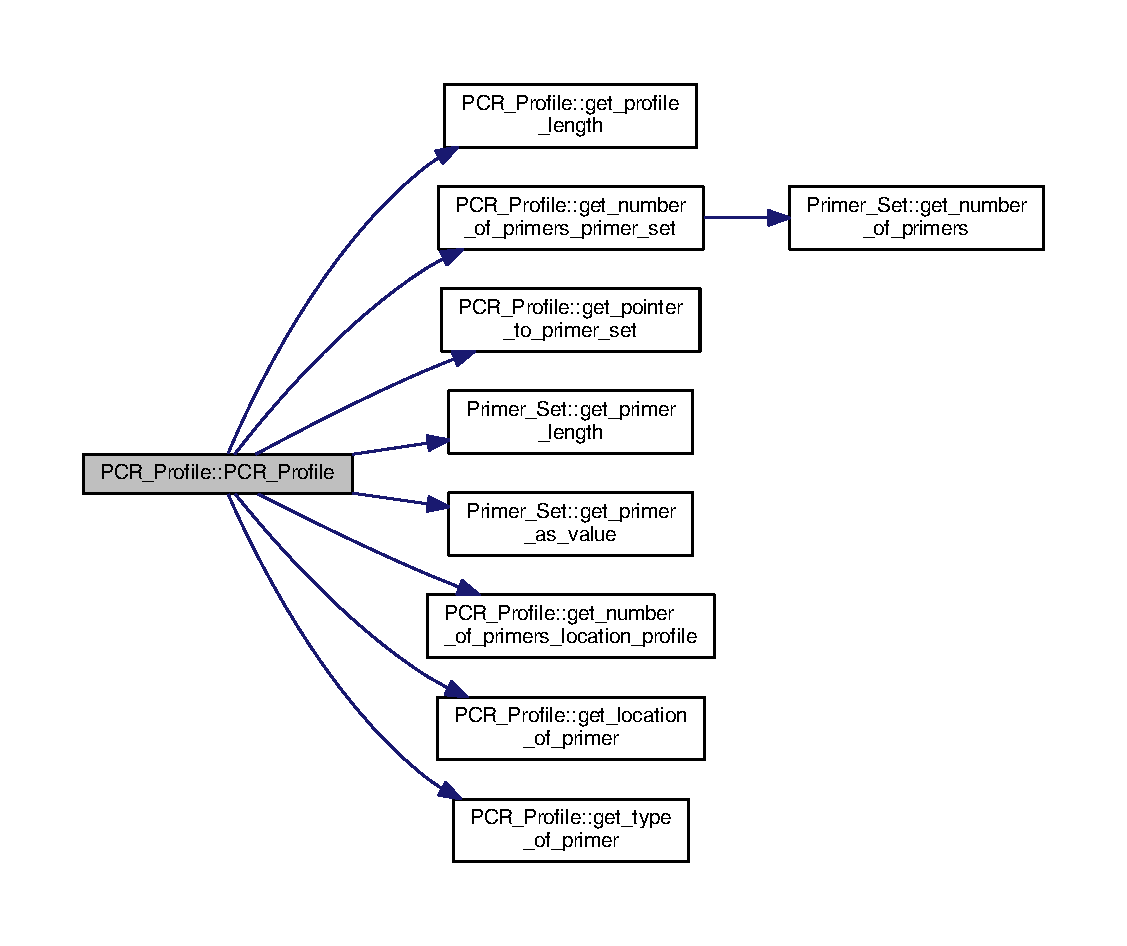
\includegraphics[width=350pt]{class_p_c_r___profile_a3b52a78e4b4db8f2c571aaf66bf9a2cc_cgraph}
\end{center}
\end{figure}
\mbox{\Hypertarget{class_p_c_r___profile_a4b621dd306d51186d84ac65929f14e7b}\label{class_p_c_r___profile_a4b621dd306d51186d84ac65929f14e7b}} 
\index{P\+C\+R\+\_\+\+Profile@{P\+C\+R\+\_\+\+Profile}!P\+C\+R\+\_\+\+Profile@{P\+C\+R\+\_\+\+Profile}}
\index{P\+C\+R\+\_\+\+Profile@{P\+C\+R\+\_\+\+Profile}!P\+C\+R\+\_\+\+Profile@{P\+C\+R\+\_\+\+Profile}}
\subsubsection{\texorpdfstring{P\+C\+R\+\_\+\+Profile()}{PCR\_Profile()}\hspace{0.1cm}{\footnotesize\ttfamily [2/3]}}
{\footnotesize\ttfamily P\+C\+R\+\_\+\+Profile\+::\+P\+C\+R\+\_\+\+Profile (\begin{DoxyParamCaption}\item[{\mbox{\hyperlink{class_p_c_r___profile}{P\+C\+R\+\_\+\+Profile}} $\ast$}]{\+\_\+pcr\+\_\+profile,  }\item[{ostream \&}]{err\+\_\+msg = {\ttfamily cout} }\end{DoxyParamCaption})}



Definition at line 194 of file P\+C\+R\+\_\+\+Profile.\+h.

Here is the call graph for this function\+:
\nopagebreak
\begin{figure}[H]
\begin{center}
\leavevmode
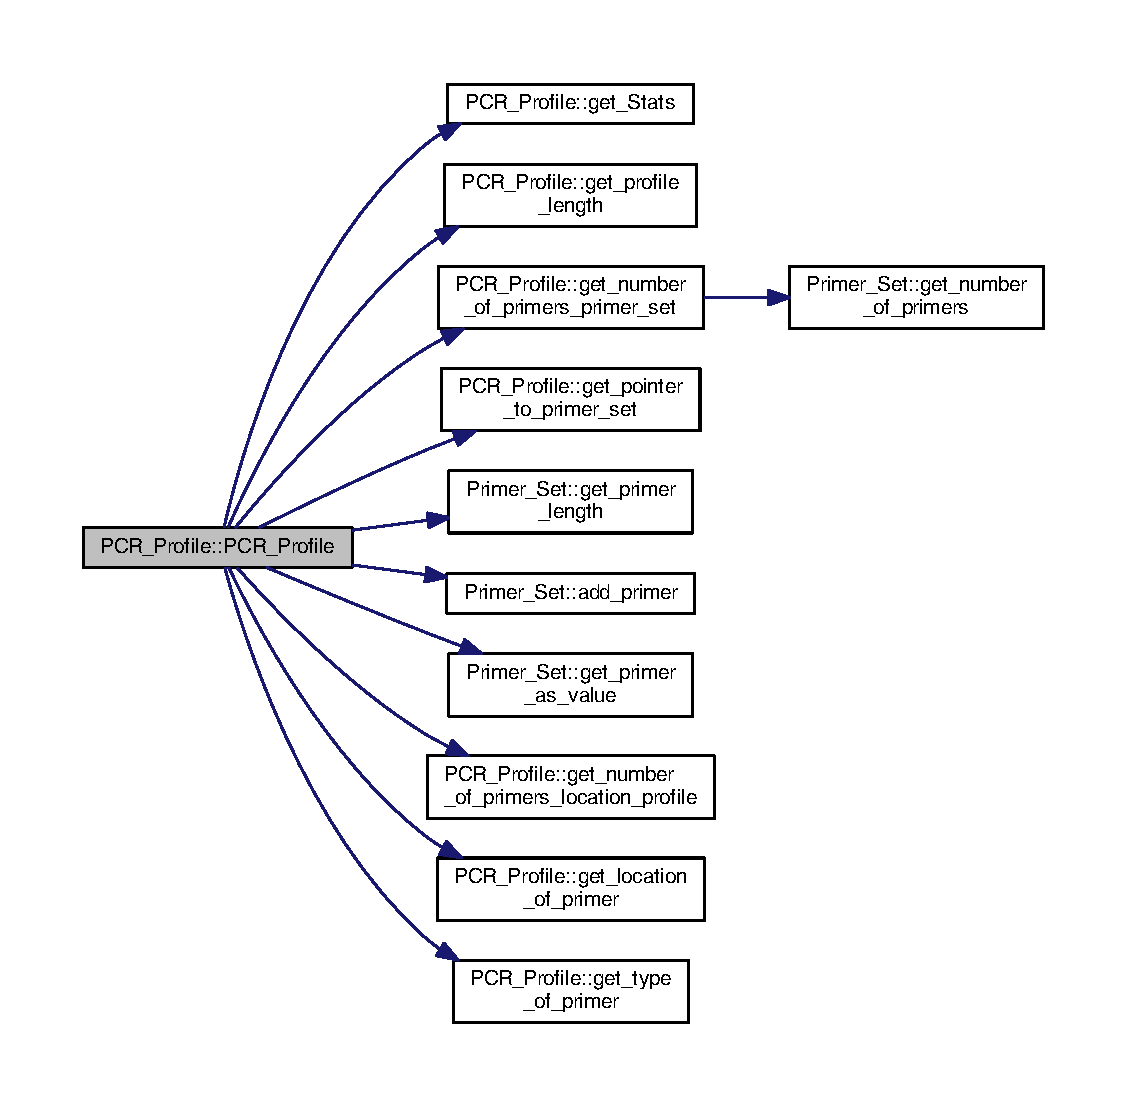
\includegraphics[width=350pt]{class_p_c_r___profile_a4b621dd306d51186d84ac65929f14e7b_cgraph}
\end{center}
\end{figure}
\mbox{\Hypertarget{class_p_c_r___profile_a2772873e5a43e8b8c1dde4b6ca9d8a2f}\label{class_p_c_r___profile_a2772873e5a43e8b8c1dde4b6ca9d8a2f}} 
\index{P\+C\+R\+\_\+\+Profile@{P\+C\+R\+\_\+\+Profile}!P\+C\+R\+\_\+\+Profile@{P\+C\+R\+\_\+\+Profile}}
\index{P\+C\+R\+\_\+\+Profile@{P\+C\+R\+\_\+\+Profile}!P\+C\+R\+\_\+\+Profile@{P\+C\+R\+\_\+\+Profile}}
\subsubsection{\texorpdfstring{P\+C\+R\+\_\+\+Profile()}{PCR\_Profile()}\hspace{0.1cm}{\footnotesize\ttfamily [3/3]}}
{\footnotesize\ttfamily P\+C\+R\+\_\+\+Profile\+::\+P\+C\+R\+\_\+\+Profile (\begin{DoxyParamCaption}\item[{\mbox{\hyperlink{class_primer___set}{Primer\+\_\+\+Set}} $\ast$}]{\+\_\+primer\+\_\+set,  }\item[{\mbox{\hyperlink{class_sequence}{Sequence}} $\ast$}]{\+\_\+sequence,  }\item[{ostream \&}]{err\+\_\+msg = {\ttfamily cout} }\end{DoxyParamCaption})}



Definition at line 225 of file P\+C\+R\+\_\+\+Profile.\+h.

Here is the call graph for this function\+:
\nopagebreak
\begin{figure}[H]
\begin{center}
\leavevmode
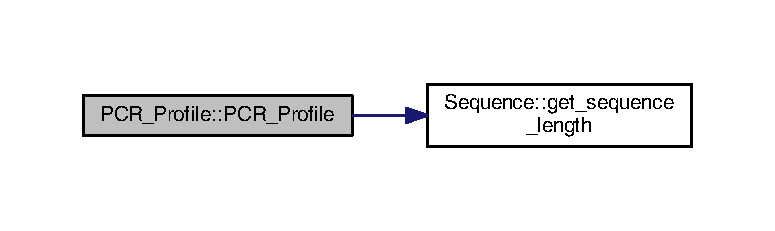
\includegraphics[width=350pt]{class_p_c_r___profile_a2772873e5a43e8b8c1dde4b6ca9d8a2f_cgraph}
\end{center}
\end{figure}
\mbox{\Hypertarget{class_p_c_r___profile_a0e83f85f3689ebd7c07005dd8440b185}\label{class_p_c_r___profile_a0e83f85f3689ebd7c07005dd8440b185}} 
\index{P\+C\+R\+\_\+\+Profile@{P\+C\+R\+\_\+\+Profile}!````~P\+C\+R\+\_\+\+Profile@{$\sim$\+P\+C\+R\+\_\+\+Profile}}
\index{````~P\+C\+R\+\_\+\+Profile@{$\sim$\+P\+C\+R\+\_\+\+Profile}!P\+C\+R\+\_\+\+Profile@{P\+C\+R\+\_\+\+Profile}}
\subsubsection{\texorpdfstring{$\sim$\+P\+C\+R\+\_\+\+Profile()}{~PCR\_Profile()}}
{\footnotesize\ttfamily P\+C\+R\+\_\+\+Profile\+::$\sim$\+P\+C\+R\+\_\+\+Profile (\begin{DoxyParamCaption}{ }\end{DoxyParamCaption})}



Definition at line 76 of file P\+C\+R\+\_\+\+Profile.\+h.



\subsection{Member Function Documentation}
\mbox{\Hypertarget{class_p_c_r___profile_a95758e5dff688b7b85bd1009ba28e112}\label{class_p_c_r___profile_a95758e5dff688b7b85bd1009ba28e112}} 
\index{P\+C\+R\+\_\+\+Profile@{P\+C\+R\+\_\+\+Profile}!add\+\_\+primer\+\_\+location\+\_\+to\+\_\+profile@{add\+\_\+primer\+\_\+location\+\_\+to\+\_\+profile}}
\index{add\+\_\+primer\+\_\+location\+\_\+to\+\_\+profile@{add\+\_\+primer\+\_\+location\+\_\+to\+\_\+profile}!P\+C\+R\+\_\+\+Profile@{P\+C\+R\+\_\+\+Profile}}
\subsubsection{\texorpdfstring{add\+\_\+primer\+\_\+location\+\_\+to\+\_\+profile()}{add\_primer\_location\_to\_profile()}}
{\footnotesize\ttfamily bool P\+C\+R\+\_\+\+Profile\+::add\+\_\+primer\+\_\+location\+\_\+to\+\_\+profile (\begin{DoxyParamCaption}\item[{unsigned int}]{position,  }\item[{int}]{primer\+\_\+type,  }\item[{ostream \&}]{err\+\_\+msg = {\ttfamily cout} }\end{DoxyParamCaption})}



Definition at line 252 of file P\+C\+R\+\_\+\+Profile.\+h.

\mbox{\Hypertarget{class_p_c_r___profile_a6f209d643d15a15c7a7b940e18df9497}\label{class_p_c_r___profile_a6f209d643d15a15c7a7b940e18df9497}} 
\index{P\+C\+R\+\_\+\+Profile@{P\+C\+R\+\_\+\+Profile}!calculate\+\_\+statistics@{calculate\+\_\+statistics}}
\index{calculate\+\_\+statistics@{calculate\+\_\+statistics}!P\+C\+R\+\_\+\+Profile@{P\+C\+R\+\_\+\+Profile}}
\subsubsection{\texorpdfstring{calculate\+\_\+statistics()}{calculate\_statistics()}}
{\footnotesize\ttfamily bool P\+C\+R\+\_\+\+Profile\+::calculate\+\_\+statistics (\begin{DoxyParamCaption}\item[{ostream \&}]{out = {\ttfamily cout},  }\item[{ostream \&}]{err\+\_\+msg = {\ttfamily cout} }\end{DoxyParamCaption})}



Definition at line 327 of file P\+C\+R\+\_\+\+Profile.\+h.

\mbox{\Hypertarget{class_p_c_r___profile_a7f9b958200413a71f4edd93277da1765}\label{class_p_c_r___profile_a7f9b958200413a71f4edd93277da1765}} 
\index{P\+C\+R\+\_\+\+Profile@{P\+C\+R\+\_\+\+Profile}!get\+\_\+location\+\_\+of\+\_\+primer@{get\+\_\+location\+\_\+of\+\_\+primer}}
\index{get\+\_\+location\+\_\+of\+\_\+primer@{get\+\_\+location\+\_\+of\+\_\+primer}!P\+C\+R\+\_\+\+Profile@{P\+C\+R\+\_\+\+Profile}}
\subsubsection{\texorpdfstring{get\+\_\+location\+\_\+of\+\_\+primer()}{get\_location\_of\_primer()}}
{\footnotesize\ttfamily int$\ast$ P\+C\+R\+\_\+\+Profile\+::get\+\_\+location\+\_\+of\+\_\+primer (\begin{DoxyParamCaption}{ }\end{DoxyParamCaption})\hspace{0.3cm}{\ttfamily [inline]}}



Definition at line 66 of file P\+C\+R\+\_\+\+Profile.\+h.

Here is the caller graph for this function\+:
\nopagebreak
\begin{figure}[H]
\begin{center}
\leavevmode
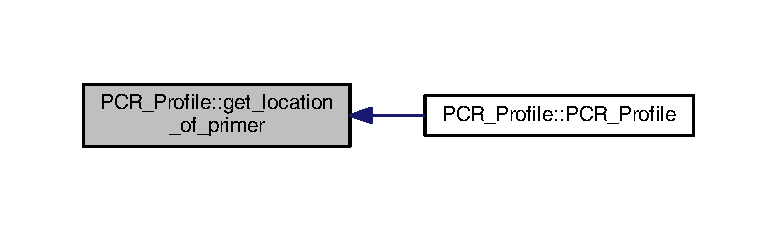
\includegraphics[width=350pt]{class_p_c_r___profile_a7f9b958200413a71f4edd93277da1765_icgraph}
\end{center}
\end{figure}
\mbox{\Hypertarget{class_p_c_r___profile_a5222753c5f4b1568f7254be8fbc7c862}\label{class_p_c_r___profile_a5222753c5f4b1568f7254be8fbc7c862}} 
\index{P\+C\+R\+\_\+\+Profile@{P\+C\+R\+\_\+\+Profile}!get\+\_\+number\+\_\+forward\+\_\+primers@{get\+\_\+number\+\_\+forward\+\_\+primers}}
\index{get\+\_\+number\+\_\+forward\+\_\+primers@{get\+\_\+number\+\_\+forward\+\_\+primers}!P\+C\+R\+\_\+\+Profile@{P\+C\+R\+\_\+\+Profile}}
\subsubsection{\texorpdfstring{get\+\_\+number\+\_\+forward\+\_\+primers()}{get\_number\_forward\_primers()}}
{\footnotesize\ttfamily unsigned int P\+C\+R\+\_\+\+Profile\+::get\+\_\+number\+\_\+forward\+\_\+primers (\begin{DoxyParamCaption}{ }\end{DoxyParamCaption})\hspace{0.3cm}{\ttfamily [inline]}}



Definition at line 53 of file P\+C\+R\+\_\+\+Profile.\+h.

\mbox{\Hypertarget{class_p_c_r___profile_a91a98d9005a63450de3f782c9374972a}\label{class_p_c_r___profile_a91a98d9005a63450de3f782c9374972a}} 
\index{P\+C\+R\+\_\+\+Profile@{P\+C\+R\+\_\+\+Profile}!get\+\_\+number\+\_\+long\+\_\+amplicons@{get\+\_\+number\+\_\+long\+\_\+amplicons}}
\index{get\+\_\+number\+\_\+long\+\_\+amplicons@{get\+\_\+number\+\_\+long\+\_\+amplicons}!P\+C\+R\+\_\+\+Profile@{P\+C\+R\+\_\+\+Profile}}
\subsubsection{\texorpdfstring{get\+\_\+number\+\_\+long\+\_\+amplicons()}{get\_number\_long\_amplicons()}}
{\footnotesize\ttfamily unsigned int P\+C\+R\+\_\+\+Profile\+::get\+\_\+number\+\_\+long\+\_\+amplicons (\begin{DoxyParamCaption}{ }\end{DoxyParamCaption})\hspace{0.3cm}{\ttfamily [inline]}}



Definition at line 56 of file P\+C\+R\+\_\+\+Profile.\+h.

\mbox{\Hypertarget{class_p_c_r___profile_a7b3b84627171a22a57366adc1992ff3d}\label{class_p_c_r___profile_a7b3b84627171a22a57366adc1992ff3d}} 
\index{P\+C\+R\+\_\+\+Profile@{P\+C\+R\+\_\+\+Profile}!get\+\_\+number\+\_\+of\+\_\+primers\+\_\+location\+\_\+profile@{get\+\_\+number\+\_\+of\+\_\+primers\+\_\+location\+\_\+profile}}
\index{get\+\_\+number\+\_\+of\+\_\+primers\+\_\+location\+\_\+profile@{get\+\_\+number\+\_\+of\+\_\+primers\+\_\+location\+\_\+profile}!P\+C\+R\+\_\+\+Profile@{P\+C\+R\+\_\+\+Profile}}
\subsubsection{\texorpdfstring{get\+\_\+number\+\_\+of\+\_\+primers\+\_\+location\+\_\+profile()}{get\_number\_of\_primers\_location\_profile()}}
{\footnotesize\ttfamily unsigned int P\+C\+R\+\_\+\+Profile\+::get\+\_\+number\+\_\+of\+\_\+primers\+\_\+location\+\_\+profile (\begin{DoxyParamCaption}{ }\end{DoxyParamCaption})\hspace{0.3cm}{\ttfamily [inline]}}



Definition at line 65 of file P\+C\+R\+\_\+\+Profile.\+h.

Here is the caller graph for this function\+:
\nopagebreak
\begin{figure}[H]
\begin{center}
\leavevmode
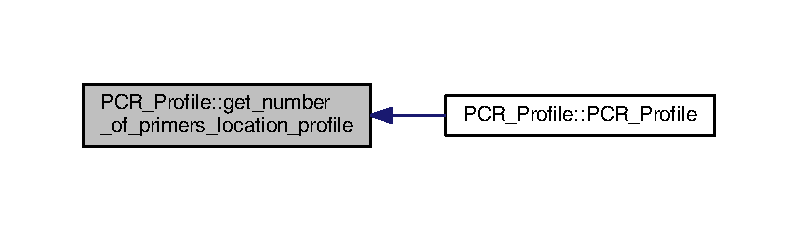
\includegraphics[width=350pt]{class_p_c_r___profile_a7b3b84627171a22a57366adc1992ff3d_icgraph}
\end{center}
\end{figure}
\mbox{\Hypertarget{class_p_c_r___profile_a3adc7245807935d0d10c7600593254a2}\label{class_p_c_r___profile_a3adc7245807935d0d10c7600593254a2}} 
\index{P\+C\+R\+\_\+\+Profile@{P\+C\+R\+\_\+\+Profile}!get\+\_\+number\+\_\+of\+\_\+primers\+\_\+primer\+\_\+set@{get\+\_\+number\+\_\+of\+\_\+primers\+\_\+primer\+\_\+set}}
\index{get\+\_\+number\+\_\+of\+\_\+primers\+\_\+primer\+\_\+set@{get\+\_\+number\+\_\+of\+\_\+primers\+\_\+primer\+\_\+set}!P\+C\+R\+\_\+\+Profile@{P\+C\+R\+\_\+\+Profile}}
\subsubsection{\texorpdfstring{get\+\_\+number\+\_\+of\+\_\+primers\+\_\+primer\+\_\+set()}{get\_number\_of\_primers\_primer\_set()}}
{\footnotesize\ttfamily unsigned int P\+C\+R\+\_\+\+Profile\+::get\+\_\+number\+\_\+of\+\_\+primers\+\_\+primer\+\_\+set (\begin{DoxyParamCaption}{ }\end{DoxyParamCaption})\hspace{0.3cm}{\ttfamily [inline]}}



Definition at line 63 of file P\+C\+R\+\_\+\+Profile.\+h.

Here is the call graph for this function\+:
\nopagebreak
\begin{figure}[H]
\begin{center}
\leavevmode
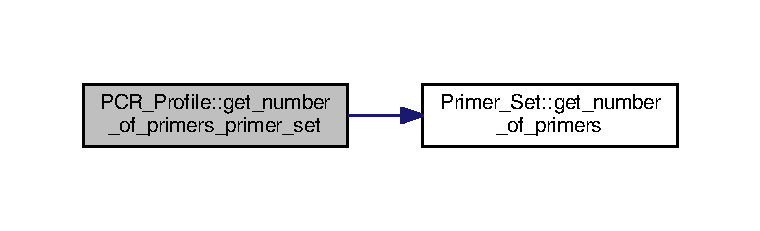
\includegraphics[width=350pt]{class_p_c_r___profile_a3adc7245807935d0d10c7600593254a2_cgraph}
\end{center}
\end{figure}
Here is the caller graph for this function\+:
\nopagebreak
\begin{figure}[H]
\begin{center}
\leavevmode
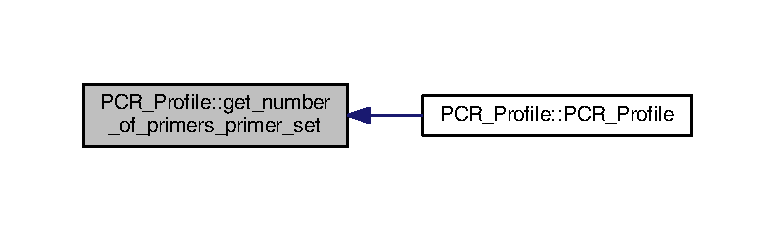
\includegraphics[width=350pt]{class_p_c_r___profile_a3adc7245807935d0d10c7600593254a2_icgraph}
\end{center}
\end{figure}
\mbox{\Hypertarget{class_p_c_r___profile_a5470c4248e9c347b66ee1ad977d2a6f9}\label{class_p_c_r___profile_a5470c4248e9c347b66ee1ad977d2a6f9}} 
\index{P\+C\+R\+\_\+\+Profile@{P\+C\+R\+\_\+\+Profile}!get\+\_\+number\+\_\+reverse\+\_\+primers@{get\+\_\+number\+\_\+reverse\+\_\+primers}}
\index{get\+\_\+number\+\_\+reverse\+\_\+primers@{get\+\_\+number\+\_\+reverse\+\_\+primers}!P\+C\+R\+\_\+\+Profile@{P\+C\+R\+\_\+\+Profile}}
\subsubsection{\texorpdfstring{get\+\_\+number\+\_\+reverse\+\_\+primers()}{get\_number\_reverse\_primers()}}
{\footnotesize\ttfamily unsigned int P\+C\+R\+\_\+\+Profile\+::get\+\_\+number\+\_\+reverse\+\_\+primers (\begin{DoxyParamCaption}{ }\end{DoxyParamCaption})\hspace{0.3cm}{\ttfamily [inline]}}



Definition at line 54 of file P\+C\+R\+\_\+\+Profile.\+h.

\mbox{\Hypertarget{class_p_c_r___profile_ae1470db4482cb29be8e29b96f913023c}\label{class_p_c_r___profile_ae1470db4482cb29be8e29b96f913023c}} 
\index{P\+C\+R\+\_\+\+Profile@{P\+C\+R\+\_\+\+Profile}!get\+\_\+number\+\_\+short\+\_\+amplicons@{get\+\_\+number\+\_\+short\+\_\+amplicons}}
\index{get\+\_\+number\+\_\+short\+\_\+amplicons@{get\+\_\+number\+\_\+short\+\_\+amplicons}!P\+C\+R\+\_\+\+Profile@{P\+C\+R\+\_\+\+Profile}}
\subsubsection{\texorpdfstring{get\+\_\+number\+\_\+short\+\_\+amplicons()}{get\_number\_short\_amplicons()}}
{\footnotesize\ttfamily unsigned int P\+C\+R\+\_\+\+Profile\+::get\+\_\+number\+\_\+short\+\_\+amplicons (\begin{DoxyParamCaption}{ }\end{DoxyParamCaption})\hspace{0.3cm}{\ttfamily [inline]}}



Definition at line 55 of file P\+C\+R\+\_\+\+Profile.\+h.

\mbox{\Hypertarget{class_p_c_r___profile_a24577af6213a4f6ae4215d19836c5673}\label{class_p_c_r___profile_a24577af6213a4f6ae4215d19836c5673}} 
\index{P\+C\+R\+\_\+\+Profile@{P\+C\+R\+\_\+\+Profile}!get\+\_\+pointer\+\_\+to\+\_\+primer\+\_\+set@{get\+\_\+pointer\+\_\+to\+\_\+primer\+\_\+set}}
\index{get\+\_\+pointer\+\_\+to\+\_\+primer\+\_\+set@{get\+\_\+pointer\+\_\+to\+\_\+primer\+\_\+set}!P\+C\+R\+\_\+\+Profile@{P\+C\+R\+\_\+\+Profile}}
\subsubsection{\texorpdfstring{get\+\_\+pointer\+\_\+to\+\_\+primer\+\_\+set()}{get\_pointer\_to\_primer\_set()}}
{\footnotesize\ttfamily \mbox{\hyperlink{class_primer___set}{Primer\+\_\+\+Set}}$\ast$ P\+C\+R\+\_\+\+Profile\+::get\+\_\+pointer\+\_\+to\+\_\+primer\+\_\+set (\begin{DoxyParamCaption}{ }\end{DoxyParamCaption})\hspace{0.3cm}{\ttfamily [inline]}}



Definition at line 62 of file P\+C\+R\+\_\+\+Profile.\+h.

Here is the caller graph for this function\+:
\nopagebreak
\begin{figure}[H]
\begin{center}
\leavevmode
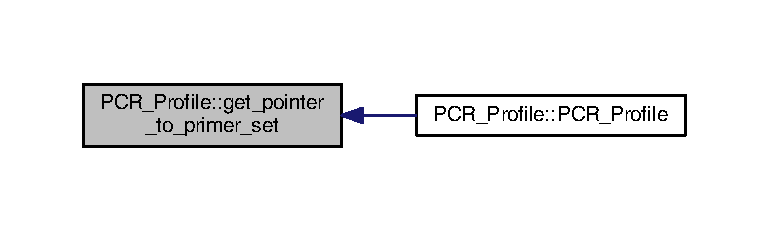
\includegraphics[width=350pt]{class_p_c_r___profile_a24577af6213a4f6ae4215d19836c5673_icgraph}
\end{center}
\end{figure}
\mbox{\Hypertarget{class_p_c_r___profile_a43b9d518bca0cd7f37ce008fcfa1b37b}\label{class_p_c_r___profile_a43b9d518bca0cd7f37ce008fcfa1b37b}} 
\index{P\+C\+R\+\_\+\+Profile@{P\+C\+R\+\_\+\+Profile}!get\+\_\+primer\+\_\+profile\+\_\+array\+\_\+size@{get\+\_\+primer\+\_\+profile\+\_\+array\+\_\+size}}
\index{get\+\_\+primer\+\_\+profile\+\_\+array\+\_\+size@{get\+\_\+primer\+\_\+profile\+\_\+array\+\_\+size}!P\+C\+R\+\_\+\+Profile@{P\+C\+R\+\_\+\+Profile}}
\subsubsection{\texorpdfstring{get\+\_\+primer\+\_\+profile\+\_\+array\+\_\+size()}{get\_primer\_profile\_array\_size()}}
{\footnotesize\ttfamily unsigned int P\+C\+R\+\_\+\+Profile\+::get\+\_\+primer\+\_\+profile\+\_\+array\+\_\+size (\begin{DoxyParamCaption}{ }\end{DoxyParamCaption})\hspace{0.3cm}{\ttfamily [inline]}}



Definition at line 64 of file P\+C\+R\+\_\+\+Profile.\+h.

\mbox{\Hypertarget{class_p_c_r___profile_ad25903940b769ad48abaf472175e5ccf}\label{class_p_c_r___profile_ad25903940b769ad48abaf472175e5ccf}} 
\index{P\+C\+R\+\_\+\+Profile@{P\+C\+R\+\_\+\+Profile}!get\+\_\+profile\+\_\+length@{get\+\_\+profile\+\_\+length}}
\index{get\+\_\+profile\+\_\+length@{get\+\_\+profile\+\_\+length}!P\+C\+R\+\_\+\+Profile@{P\+C\+R\+\_\+\+Profile}}
\subsubsection{\texorpdfstring{get\+\_\+profile\+\_\+length()}{get\_profile\_length()}}
{\footnotesize\ttfamily unsigned int P\+C\+R\+\_\+\+Profile\+::get\+\_\+profile\+\_\+length (\begin{DoxyParamCaption}{ }\end{DoxyParamCaption})\hspace{0.3cm}{\ttfamily [inline]}}



Definition at line 59 of file P\+C\+R\+\_\+\+Profile.\+h.

Here is the caller graph for this function\+:
\nopagebreak
\begin{figure}[H]
\begin{center}
\leavevmode
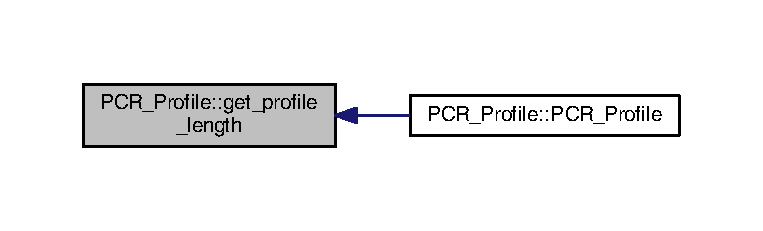
\includegraphics[width=350pt]{class_p_c_r___profile_ad25903940b769ad48abaf472175e5ccf_icgraph}
\end{center}
\end{figure}
\mbox{\Hypertarget{class_p_c_r___profile_a05e64bbe69413cb969b31ffae46e6a10}\label{class_p_c_r___profile_a05e64bbe69413cb969b31ffae46e6a10}} 
\index{P\+C\+R\+\_\+\+Profile@{P\+C\+R\+\_\+\+Profile}!get\+\_\+\+Stats@{get\+\_\+\+Stats}}
\index{get\+\_\+\+Stats@{get\+\_\+\+Stats}!P\+C\+R\+\_\+\+Profile@{P\+C\+R\+\_\+\+Profile}}
\subsubsection{\texorpdfstring{get\+\_\+\+Stats()}{get\_Stats()}}
{\footnotesize\ttfamily Stats P\+C\+R\+\_\+\+Profile\+::get\+\_\+\+Stats (\begin{DoxyParamCaption}{ }\end{DoxyParamCaption})\hspace{0.3cm}{\ttfamily [inline]}}



Definition at line 70 of file P\+C\+R\+\_\+\+Profile.\+h.

Here is the caller graph for this function\+:
\nopagebreak
\begin{figure}[H]
\begin{center}
\leavevmode
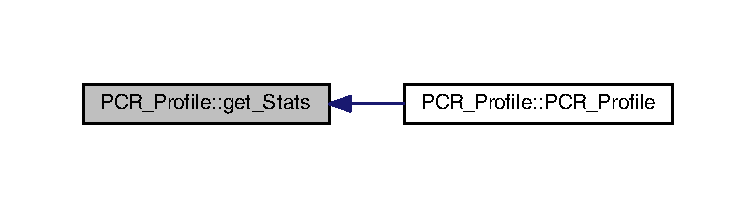
\includegraphics[width=350pt]{class_p_c_r___profile_a05e64bbe69413cb969b31ffae46e6a10_icgraph}
\end{center}
\end{figure}
\mbox{\Hypertarget{class_p_c_r___profile_adf41a697d05489582745d650d4e7c956}\label{class_p_c_r___profile_adf41a697d05489582745d650d4e7c956}} 
\index{P\+C\+R\+\_\+\+Profile@{P\+C\+R\+\_\+\+Profile}!get\+\_\+total\+\_\+lenght\+\_\+long\+\_\+amplicons@{get\+\_\+total\+\_\+lenght\+\_\+long\+\_\+amplicons}}
\index{get\+\_\+total\+\_\+lenght\+\_\+long\+\_\+amplicons@{get\+\_\+total\+\_\+lenght\+\_\+long\+\_\+amplicons}!P\+C\+R\+\_\+\+Profile@{P\+C\+R\+\_\+\+Profile}}
\subsubsection{\texorpdfstring{get\+\_\+total\+\_\+lenght\+\_\+long\+\_\+amplicons()}{get\_total\_lenght\_long\_amplicons()}}
{\footnotesize\ttfamily unsigned int P\+C\+R\+\_\+\+Profile\+::get\+\_\+total\+\_\+lenght\+\_\+long\+\_\+amplicons (\begin{DoxyParamCaption}{ }\end{DoxyParamCaption})\hspace{0.3cm}{\ttfamily [inline]}}



Definition at line 58 of file P\+C\+R\+\_\+\+Profile.\+h.

Here is the caller graph for this function\+:
\nopagebreak
\begin{figure}[H]
\begin{center}
\leavevmode
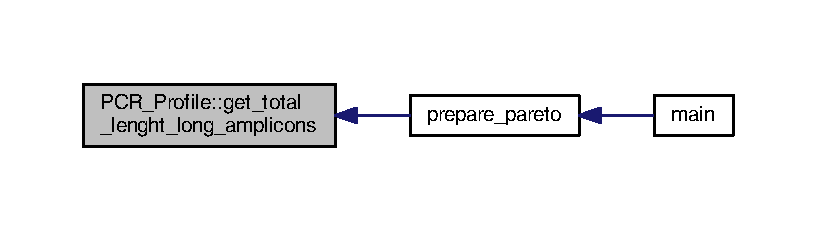
\includegraphics[width=350pt]{class_p_c_r___profile_adf41a697d05489582745d650d4e7c956_icgraph}
\end{center}
\end{figure}
\mbox{\Hypertarget{class_p_c_r___profile_aa8f3e8fc43865af8734090436a0d729e}\label{class_p_c_r___profile_aa8f3e8fc43865af8734090436a0d729e}} 
\index{P\+C\+R\+\_\+\+Profile@{P\+C\+R\+\_\+\+Profile}!get\+\_\+total\+\_\+lenght\+\_\+short\+\_\+amplicons@{get\+\_\+total\+\_\+lenght\+\_\+short\+\_\+amplicons}}
\index{get\+\_\+total\+\_\+lenght\+\_\+short\+\_\+amplicons@{get\+\_\+total\+\_\+lenght\+\_\+short\+\_\+amplicons}!P\+C\+R\+\_\+\+Profile@{P\+C\+R\+\_\+\+Profile}}
\subsubsection{\texorpdfstring{get\+\_\+total\+\_\+lenght\+\_\+short\+\_\+amplicons()}{get\_total\_lenght\_short\_amplicons()}}
{\footnotesize\ttfamily unsigned int P\+C\+R\+\_\+\+Profile\+::get\+\_\+total\+\_\+lenght\+\_\+short\+\_\+amplicons (\begin{DoxyParamCaption}{ }\end{DoxyParamCaption})\hspace{0.3cm}{\ttfamily [inline]}}



Definition at line 57 of file P\+C\+R\+\_\+\+Profile.\+h.

Here is the caller graph for this function\+:
\nopagebreak
\begin{figure}[H]
\begin{center}
\leavevmode
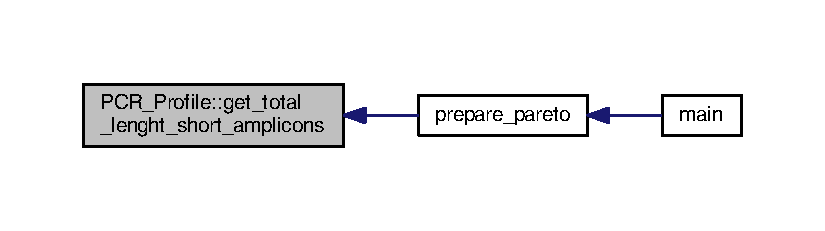
\includegraphics[width=350pt]{class_p_c_r___profile_aa8f3e8fc43865af8734090436a0d729e_icgraph}
\end{center}
\end{figure}
\mbox{\Hypertarget{class_p_c_r___profile_a0c37a463d8adedb60c5b4d8d213c182e}\label{class_p_c_r___profile_a0c37a463d8adedb60c5b4d8d213c182e}} 
\index{P\+C\+R\+\_\+\+Profile@{P\+C\+R\+\_\+\+Profile}!get\+\_\+total\+\_\+lenght\+\_\+too\+\_\+long\+\_\+amplicons@{get\+\_\+total\+\_\+lenght\+\_\+too\+\_\+long\+\_\+amplicons}}
\index{get\+\_\+total\+\_\+lenght\+\_\+too\+\_\+long\+\_\+amplicons@{get\+\_\+total\+\_\+lenght\+\_\+too\+\_\+long\+\_\+amplicons}!P\+C\+R\+\_\+\+Profile@{P\+C\+R\+\_\+\+Profile}}
\subsubsection{\texorpdfstring{get\+\_\+total\+\_\+lenght\+\_\+too\+\_\+long\+\_\+amplicons()}{get\_total\_lenght\_too\_long\_amplicons()}}
{\footnotesize\ttfamily unsigned int P\+C\+R\+\_\+\+Profile\+::get\+\_\+total\+\_\+lenght\+\_\+too\+\_\+long\+\_\+amplicons (\begin{DoxyParamCaption}{ }\end{DoxyParamCaption})\hspace{0.3cm}{\ttfamily [inline]}}



Definition at line 60 of file P\+C\+R\+\_\+\+Profile.\+h.

\mbox{\Hypertarget{class_p_c_r___profile_abcd1baf20c93c633b00b1fbd3e662b8f}\label{class_p_c_r___profile_abcd1baf20c93c633b00b1fbd3e662b8f}} 
\index{P\+C\+R\+\_\+\+Profile@{P\+C\+R\+\_\+\+Profile}!get\+\_\+total\+\_\+length\+\_\+uncovered@{get\+\_\+total\+\_\+length\+\_\+uncovered}}
\index{get\+\_\+total\+\_\+length\+\_\+uncovered@{get\+\_\+total\+\_\+length\+\_\+uncovered}!P\+C\+R\+\_\+\+Profile@{P\+C\+R\+\_\+\+Profile}}
\subsubsection{\texorpdfstring{get\+\_\+total\+\_\+length\+\_\+uncovered()}{get\_total\_length\_uncovered()}}
{\footnotesize\ttfamily unsigned int P\+C\+R\+\_\+\+Profile\+::get\+\_\+total\+\_\+length\+\_\+uncovered (\begin{DoxyParamCaption}{ }\end{DoxyParamCaption})\hspace{0.3cm}{\ttfamily [inline]}}



Definition at line 61 of file P\+C\+R\+\_\+\+Profile.\+h.

\mbox{\Hypertarget{class_p_c_r___profile_a6243b3536533df498c781f9e592a86db}\label{class_p_c_r___profile_a6243b3536533df498c781f9e592a86db}} 
\index{P\+C\+R\+\_\+\+Profile@{P\+C\+R\+\_\+\+Profile}!get\+\_\+type\+\_\+of\+\_\+primer@{get\+\_\+type\+\_\+of\+\_\+primer}}
\index{get\+\_\+type\+\_\+of\+\_\+primer@{get\+\_\+type\+\_\+of\+\_\+primer}!P\+C\+R\+\_\+\+Profile@{P\+C\+R\+\_\+\+Profile}}
\subsubsection{\texorpdfstring{get\+\_\+type\+\_\+of\+\_\+primer()}{get\_type\_of\_primer()}}
{\footnotesize\ttfamily int$\ast$ P\+C\+R\+\_\+\+Profile\+::get\+\_\+type\+\_\+of\+\_\+primer (\begin{DoxyParamCaption}{ }\end{DoxyParamCaption})\hspace{0.3cm}{\ttfamily [inline]}}



Definition at line 67 of file P\+C\+R\+\_\+\+Profile.\+h.

Here is the caller graph for this function\+:
\nopagebreak
\begin{figure}[H]
\begin{center}
\leavevmode
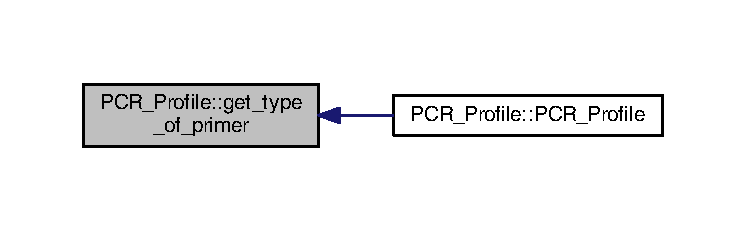
\includegraphics[width=350pt]{class_p_c_r___profile_a6243b3536533df498c781f9e592a86db_icgraph}
\end{center}
\end{figure}
\mbox{\Hypertarget{class_p_c_r___profile_a339a01da69e5e709f6b33678bd9f73dc}\label{class_p_c_r___profile_a339a01da69e5e709f6b33678bd9f73dc}} 
\index{P\+C\+R\+\_\+\+Profile@{P\+C\+R\+\_\+\+Profile}!P\+C\+R\+\_\+profile\+\_\+calculation@{P\+C\+R\+\_\+profile\+\_\+calculation}}
\index{P\+C\+R\+\_\+profile\+\_\+calculation@{P\+C\+R\+\_\+profile\+\_\+calculation}!P\+C\+R\+\_\+\+Profile@{P\+C\+R\+\_\+\+Profile}}
\subsubsection{\texorpdfstring{P\+C\+R\+\_\+profile\+\_\+calculation()}{PCR\_profile\_calculation()}}
{\footnotesize\ttfamily bool P\+C\+R\+\_\+\+Profile\+::\+P\+C\+R\+\_\+profile\+\_\+calculation (\begin{DoxyParamCaption}\item[{\mbox{\hyperlink{class_sequence}{Sequence}} $\ast$}]{\+\_\+sequence,  }\item[{ostream \&}]{err\+\_\+msg = {\ttfamily cout} }\end{DoxyParamCaption})}



Definition at line 299 of file P\+C\+R\+\_\+\+Profile.\+h.

Here is the call graph for this function\+:
\nopagebreak
\begin{figure}[H]
\begin{center}
\leavevmode
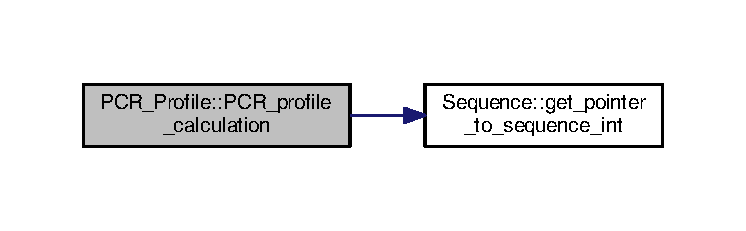
\includegraphics[width=350pt]{class_p_c_r___profile_a339a01da69e5e709f6b33678bd9f73dc_cgraph}
\end{center}
\end{figure}
\mbox{\Hypertarget{class_p_c_r___profile_aad744529e3bbcdc019d259667460340b}\label{class_p_c_r___profile_aad744529e3bbcdc019d259667460340b}} 
\index{P\+C\+R\+\_\+\+Profile@{P\+C\+R\+\_\+\+Profile}!show\+\_\+\+All@{show\+\_\+\+All}}
\index{show\+\_\+\+All@{show\+\_\+\+All}!P\+C\+R\+\_\+\+Profile@{P\+C\+R\+\_\+\+Profile}}
\subsubsection{\texorpdfstring{show\+\_\+\+All()}{show\_All()}}
{\footnotesize\ttfamily bool P\+C\+R\+\_\+\+Profile\+::show\+\_\+\+All (\begin{DoxyParamCaption}\item[{ostream \&}]{out = {\ttfamily cout},  }\item[{ostream \&}]{err\+\_\+msg = {\ttfamily cout} }\end{DoxyParamCaption})}



Definition at line 288 of file P\+C\+R\+\_\+\+Profile.\+h.

\mbox{\Hypertarget{class_p_c_r___profile_a9897676b415905e30809e69c399a859a}\label{class_p_c_r___profile_a9897676b415905e30809e69c399a859a}} 
\index{P\+C\+R\+\_\+\+Profile@{P\+C\+R\+\_\+\+Profile}!show\+\_\+statistics@{show\+\_\+statistics}}
\index{show\+\_\+statistics@{show\+\_\+statistics}!P\+C\+R\+\_\+\+Profile@{P\+C\+R\+\_\+\+Profile}}
\subsubsection{\texorpdfstring{show\+\_\+statistics()}{show\_statistics()}}
{\footnotesize\ttfamily bool P\+C\+R\+\_\+\+Profile\+::show\+\_\+statistics (\begin{DoxyParamCaption}\item[{ostream \&}]{out = {\ttfamily cout},  }\item[{ostream \&}]{err\+\_\+msg = {\ttfamily cout} }\end{DoxyParamCaption})}



Definition at line 271 of file P\+C\+R\+\_\+\+Profile.\+h.

Here is the caller graph for this function\+:
\nopagebreak
\begin{figure}[H]
\begin{center}
\leavevmode
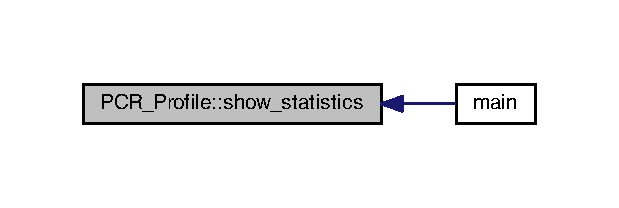
\includegraphics[width=297pt]{class_p_c_r___profile_a9897676b415905e30809e69c399a859a_icgraph}
\end{center}
\end{figure}


The documentation for this class was generated from the following file\+:\begin{DoxyCompactItemize}
\item 
R\+P\+A/\mbox{\hyperlink{_p_c_r___profile_8h}{P\+C\+R\+\_\+\+Profile.\+h}}\end{DoxyCompactItemize}

\hypertarget{class_p_c_r___profile___toolbox}{}\section{P\+C\+R\+\_\+\+Profile\+\_\+\+Toolbox Class Reference}
\label{class_p_c_r___profile___toolbox}\index{P\+C\+R\+\_\+\+Profile\+\_\+\+Toolbox@{P\+C\+R\+\_\+\+Profile\+\_\+\+Toolbox}}
\subsection*{Static Public Member Functions}
\begin{DoxyCompactItemize}
\item 
\mbox{\Hypertarget{class_p_c_r___profile___toolbox_a464d4e49e62837b23870850445fb4bcb}\label{class_p_c_r___profile___toolbox_a464d4e49e62837b23870850445fb4bcb}} 
static bool {\bfseries merge\+\_\+pcr\+\_\+profiles} (\mbox{\hyperlink{class_p_c_r___profile}{P\+C\+R\+\_\+\+Profile}} $\ast$\&resulting, \mbox{\hyperlink{class_p_c_r___profile}{P\+C\+R\+\_\+\+Profile}} $\ast$input\+\_\+a, \mbox{\hyperlink{class_p_c_r___profile}{P\+C\+R\+\_\+\+Profile}} $\ast$input\+\_\+b, ostream \&err\+\_\+msg=cout)
\item 
\mbox{\Hypertarget{class_p_c_r___profile___toolbox_a76b955a9a945af8160e34bfa03949841}\label{class_p_c_r___profile___toolbox_a76b955a9a945af8160e34bfa03949841}} 
static bool {\bfseries convert\+\_\+primer\+\_\+txt\+\_\+to\+\_\+int} (char $\ast$\+\_\+primer, unsigned int primer\+\_\+length, unsigned int \&primer\+\_\+value, ostream \&err\+\_\+msg=cout)
\end{DoxyCompactItemize}


The documentation for this class was generated from the following file\+:\begin{DoxyCompactItemize}
\item 
C\+:/\+Users/\+Kamil/\+Documents/\+R\+P\+A-\/\+Optimization/\+R\+P\+A/P\+C\+R\+\_\+\+Profile\+\_\+\+Toolbox.\+h\end{DoxyCompactItemize}

\hypertarget{class_primer___set}{}\section{Primer\+\_\+\+Set Class Reference}
\label{class_primer___set}\index{Primer\+\_\+\+Set@{Primer\+\_\+\+Set}}


{\ttfamily \#include $<$Primer\+\_\+\+Set.\+h$>$}

\subsection*{Public Member Functions}
\begin{DoxyCompactItemize}
\item 
\mbox{\hyperlink{class_primer___set_ab9db4a9ad37106aac40762b7b4d57d4f}{Primer\+\_\+\+Set}} (unsigned int array\+\_\+size\+\_\+primers, unsigned int \+\_\+primer\+\_\+length, ostream \&err\+\_\+msg=cout)
\item 
\mbox{\hyperlink{class_primer___set_ae81dafc2ac39deb5480f68dac440e88e}{Primer\+\_\+\+Set}} (char $\ast$filename, ostream \&err\+\_\+msg=cout)
\item 
\mbox{\hyperlink{class_primer___set_a47c64ebda73f5a9d34d68f3c116c09cf}{Primer\+\_\+\+Set}} (\mbox{\hyperlink{class_primer___set}{Primer\+\_\+\+Set}} $\ast$primer\+\_\+set, ostream \&err\+\_\+msg=cout)
\item 
\mbox{\hyperlink{class_primer___set_ae3c919cd6aa18e8e2c3e4f5d3ea9a37c}{Primer\+\_\+\+Set}} (unsigned int $\ast$primers, unsigned int number\+\_\+primers, unsigned int \+\_\+max\+\_\+number\+\_\+of\+\_\+primers, ostream \&err\+\_\+msg=cout)
\item 
\mbox{\hyperlink{class_primer___set_aa6e3ae72bc7cd4506b48b09e6591bd0f}{Primer\+\_\+\+Set}} (char $\ast$$\ast$primers, unsigned int number\+\_\+primers, unsigned int \+\_\+max\+\_\+number\+\_\+of\+\_\+primers, ostream \&err\+\_\+msg=cout)
\item 
\mbox{\hyperlink{class_primer___set_aaeefdfa29c69f847f033b47eb43d4e05}{$\sim$\+Primer\+\_\+\+Set}} ()
\item 
bool \mbox{\hyperlink{class_primer___set_a55d08f895a8af207b7e06abf8bf95f99}{write\+\_\+to\+\_\+file}} (char $\ast$filename, ostream \&err\+\_\+msg=cout)
\item 
bool \mbox{\hyperlink{class_primer___set_a86da618d3bafd760ceb21099b168e54c}{show\+\_\+statistics}} (ostream \&out=cout, ostream \&err\+\_\+msg=cout)
\item 
bool \mbox{\hyperlink{class_primer___set_aca0009d54b4b99a0a45d4e4995bb9818}{show\+\_\+\+All}} (ostream \&out=cout, ostream \&err\+\_\+msg=cout)
\item 
unsigned int \mbox{\hyperlink{class_primer___set_a7c639e643b36dea739026862f12a64d4}{get\+\_\+primer\+\_\+as\+\_\+value}} (unsigned int position)
\item 
bool \mbox{\hyperlink{class_primer___set_a1285be11e09dff32a28e8c36d01175c5}{delete\+\_\+primer}} (int $\ast$position, unsigned int number\+\_\+of\+\_\+primers\+\_\+to\+\_\+delete, ostream \&err\+\_\+msg=cout)
\item 
bool \mbox{\hyperlink{class_primer___set_a136e11664762cb801c833209a68204fe}{add\+\_\+primer}} (unsigned int primer\+\_\+value, ostream \&err\+\_\+msg=cout)
\item 
bool \mbox{\hyperlink{class_primer___set_acbbf2f8583751542a18f895e44643be2}{add\+\_\+primer}} (char $\ast$primer, ostream \&err\+\_\+msg=cout)
\item 
bool \mbox{\hyperlink{class_primer___set_af45de3f0a9a7cac592aa66e15f1d6155}{convert\+\_\+primer\+\_\+int\+\_\+to\+\_\+txt}} (unsigned int primer\+\_\+value, char $\ast$\&primer, ostream \&err\+\_\+msg=cout)
\item 
bool \mbox{\hyperlink{class_primer___set_a0691f55ba1bb6e1dca8fcd5cdfd6bd1a}{convert\+\_\+primer\+\_\+txt\+\_\+to\+\_\+int}} (char $\ast$primer, unsigned int \&primer\+\_\+value, ostream \&err\+\_\+msg=cout)
\item 
unsigned int \mbox{\hyperlink{class_primer___set_a6f351e7eb9dc3ceb42beb4fcd368e616}{convert\+\_\+primer\+\_\+to\+\_\+reverse\+\_\+complement}} (int position, ostream \&err\+\_\+msg=cout)
\item 
unsigned int $\ast$ \mbox{\hyperlink{class_primer___set_a4eae0937a142b6399cf5b4022f8897df}{get\+\_\+pointer\+\_\+to\+\_\+primer\+\_\+array}} ()
\item 
unsigned int $\ast$ \mbox{\hyperlink{class_primer___set_ae795b4d40b4da9856b467f09462769e1}{get\+\_\+pointer\+\_\+to\+\_\+reverse\+\_\+complement\+\_\+primer\+\_\+array}} ()
\item 
unsigned int \mbox{\hyperlink{class_primer___set_af9cc2185ff8cb758f383481d138faf8f}{get\+\_\+number\+\_\+of\+\_\+primers}} ()
\item 
unsigned int \mbox{\hyperlink{class_primer___set_af53fe2ae85933f04a5cc2e159a3ed49f}{get\+\_\+primer\+\_\+length}} ()
\end{DoxyCompactItemize}


\subsection{Detailed Description}


Definition at line 16 of file Primer\+\_\+\+Set.\+h.



\subsection{Constructor \& Destructor Documentation}
\mbox{\Hypertarget{class_primer___set_ab9db4a9ad37106aac40762b7b4d57d4f}\label{class_primer___set_ab9db4a9ad37106aac40762b7b4d57d4f}} 
\index{Primer\+\_\+\+Set@{Primer\+\_\+\+Set}!Primer\+\_\+\+Set@{Primer\+\_\+\+Set}}
\index{Primer\+\_\+\+Set@{Primer\+\_\+\+Set}!Primer\+\_\+\+Set@{Primer\+\_\+\+Set}}
\subsubsection{\texorpdfstring{Primer\+\_\+\+Set()}{Primer\_Set()}\hspace{0.1cm}{\footnotesize\ttfamily [1/5]}}
{\footnotesize\ttfamily Primer\+\_\+\+Set\+::\+Primer\+\_\+\+Set (\begin{DoxyParamCaption}\item[{unsigned int}]{array\+\_\+size\+\_\+primers,  }\item[{unsigned int}]{\+\_\+primer\+\_\+length,  }\item[{ostream \&}]{err\+\_\+msg = {\ttfamily cout} }\end{DoxyParamCaption})}



Definition at line 69 of file Primer\+\_\+\+Set.\+h.

\mbox{\Hypertarget{class_primer___set_ae81dafc2ac39deb5480f68dac440e88e}\label{class_primer___set_ae81dafc2ac39deb5480f68dac440e88e}} 
\index{Primer\+\_\+\+Set@{Primer\+\_\+\+Set}!Primer\+\_\+\+Set@{Primer\+\_\+\+Set}}
\index{Primer\+\_\+\+Set@{Primer\+\_\+\+Set}!Primer\+\_\+\+Set@{Primer\+\_\+\+Set}}
\subsubsection{\texorpdfstring{Primer\+\_\+\+Set()}{Primer\_Set()}\hspace{0.1cm}{\footnotesize\ttfamily [2/5]}}
{\footnotesize\ttfamily Primer\+\_\+\+Set\+::\+Primer\+\_\+\+Set (\begin{DoxyParamCaption}\item[{char $\ast$}]{filename,  }\item[{ostream \&}]{err\+\_\+msg = {\ttfamily cout} }\end{DoxyParamCaption})}



Definition at line 104 of file Primer\+\_\+\+Set.\+h.

Here is the call graph for this function\+:
\nopagebreak
\begin{figure}[H]
\begin{center}
\leavevmode
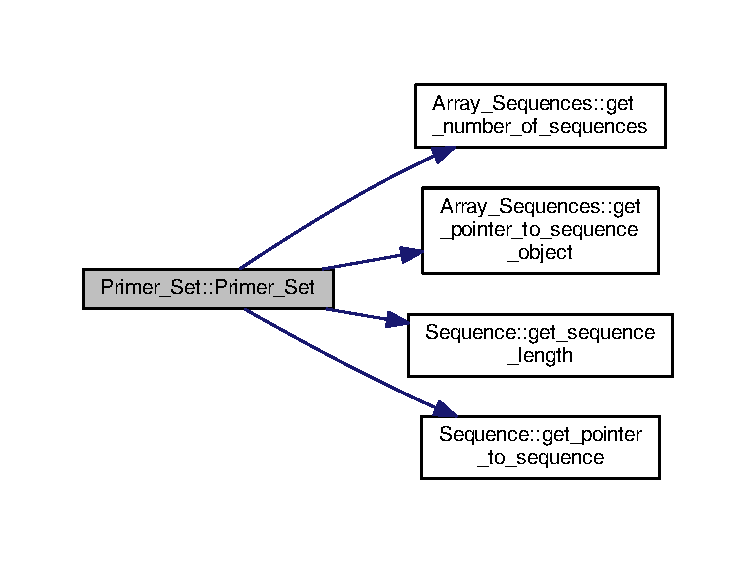
\includegraphics[width=350pt]{class_primer___set_ae81dafc2ac39deb5480f68dac440e88e_cgraph}
\end{center}
\end{figure}
\mbox{\Hypertarget{class_primer___set_a47c64ebda73f5a9d34d68f3c116c09cf}\label{class_primer___set_a47c64ebda73f5a9d34d68f3c116c09cf}} 
\index{Primer\+\_\+\+Set@{Primer\+\_\+\+Set}!Primer\+\_\+\+Set@{Primer\+\_\+\+Set}}
\index{Primer\+\_\+\+Set@{Primer\+\_\+\+Set}!Primer\+\_\+\+Set@{Primer\+\_\+\+Set}}
\subsubsection{\texorpdfstring{Primer\+\_\+\+Set()}{Primer\_Set()}\hspace{0.1cm}{\footnotesize\ttfamily [3/5]}}
{\footnotesize\ttfamily Primer\+\_\+\+Set\+::\+Primer\+\_\+\+Set (\begin{DoxyParamCaption}\item[{\mbox{\hyperlink{class_primer___set}{Primer\+\_\+\+Set}} $\ast$}]{primer\+\_\+set,  }\item[{ostream \&}]{err\+\_\+msg = {\ttfamily cout} }\end{DoxyParamCaption})}



Definition at line 78 of file Primer\+\_\+\+Set.\+h.

Here is the call graph for this function\+:
\nopagebreak
\begin{figure}[H]
\begin{center}
\leavevmode
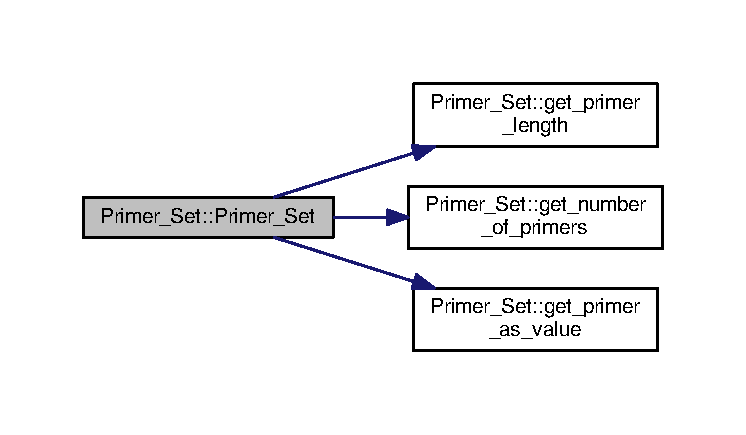
\includegraphics[width=350pt]{class_primer___set_a47c64ebda73f5a9d34d68f3c116c09cf_cgraph}
\end{center}
\end{figure}
\mbox{\Hypertarget{class_primer___set_ae3c919cd6aa18e8e2c3e4f5d3ea9a37c}\label{class_primer___set_ae3c919cd6aa18e8e2c3e4f5d3ea9a37c}} 
\index{Primer\+\_\+\+Set@{Primer\+\_\+\+Set}!Primer\+\_\+\+Set@{Primer\+\_\+\+Set}}
\index{Primer\+\_\+\+Set@{Primer\+\_\+\+Set}!Primer\+\_\+\+Set@{Primer\+\_\+\+Set}}
\subsubsection{\texorpdfstring{Primer\+\_\+\+Set()}{Primer\_Set()}\hspace{0.1cm}{\footnotesize\ttfamily [4/5]}}
{\footnotesize\ttfamily Primer\+\_\+\+Set\+::\+Primer\+\_\+\+Set (\begin{DoxyParamCaption}\item[{unsigned int $\ast$}]{primers,  }\item[{unsigned int}]{number\+\_\+primers,  }\item[{unsigned int}]{\+\_\+max\+\_\+number\+\_\+of\+\_\+primers,  }\item[{ostream \&}]{err\+\_\+msg = {\ttfamily cout} }\end{DoxyParamCaption})}

\mbox{\Hypertarget{class_primer___set_aa6e3ae72bc7cd4506b48b09e6591bd0f}\label{class_primer___set_aa6e3ae72bc7cd4506b48b09e6591bd0f}} 
\index{Primer\+\_\+\+Set@{Primer\+\_\+\+Set}!Primer\+\_\+\+Set@{Primer\+\_\+\+Set}}
\index{Primer\+\_\+\+Set@{Primer\+\_\+\+Set}!Primer\+\_\+\+Set@{Primer\+\_\+\+Set}}
\subsubsection{\texorpdfstring{Primer\+\_\+\+Set()}{Primer\_Set()}\hspace{0.1cm}{\footnotesize\ttfamily [5/5]}}
{\footnotesize\ttfamily Primer\+\_\+\+Set\+::\+Primer\+\_\+\+Set (\begin{DoxyParamCaption}\item[{char $\ast$$\ast$}]{primers,  }\item[{unsigned int}]{number\+\_\+primers,  }\item[{unsigned int}]{\+\_\+max\+\_\+number\+\_\+of\+\_\+primers,  }\item[{ostream \&}]{err\+\_\+msg = {\ttfamily cout} }\end{DoxyParamCaption})}

\mbox{\Hypertarget{class_primer___set_aaeefdfa29c69f847f033b47eb43d4e05}\label{class_primer___set_aaeefdfa29c69f847f033b47eb43d4e05}} 
\index{Primer\+\_\+\+Set@{Primer\+\_\+\+Set}!````~Primer\+\_\+\+Set@{$\sim$\+Primer\+\_\+\+Set}}
\index{````~Primer\+\_\+\+Set@{$\sim$\+Primer\+\_\+\+Set}!Primer\+\_\+\+Set@{Primer\+\_\+\+Set}}
\subsubsection{\texorpdfstring{$\sim$\+Primer\+\_\+\+Set()}{~Primer\_Set()}}
{\footnotesize\ttfamily Primer\+\_\+\+Set\+::$\sim$\+Primer\+\_\+\+Set (\begin{DoxyParamCaption}{ }\end{DoxyParamCaption})}



Definition at line 64 of file Primer\+\_\+\+Set.\+h.



\subsection{Member Function Documentation}
\mbox{\Hypertarget{class_primer___set_a136e11664762cb801c833209a68204fe}\label{class_primer___set_a136e11664762cb801c833209a68204fe}} 
\index{Primer\+\_\+\+Set@{Primer\+\_\+\+Set}!add\+\_\+primer@{add\+\_\+primer}}
\index{add\+\_\+primer@{add\+\_\+primer}!Primer\+\_\+\+Set@{Primer\+\_\+\+Set}}
\subsubsection{\texorpdfstring{add\+\_\+primer()}{add\_primer()}\hspace{0.1cm}{\footnotesize\ttfamily [1/2]}}
{\footnotesize\ttfamily bool Primer\+\_\+\+Set\+::add\+\_\+primer (\begin{DoxyParamCaption}\item[{unsigned int}]{primer\+\_\+value,  }\item[{ostream \&}]{err\+\_\+msg = {\ttfamily cout} }\end{DoxyParamCaption})}



Definition at line 267 of file Primer\+\_\+\+Set.\+h.

Here is the caller graph for this function\+:
\nopagebreak
\begin{figure}[H]
\begin{center}
\leavevmode
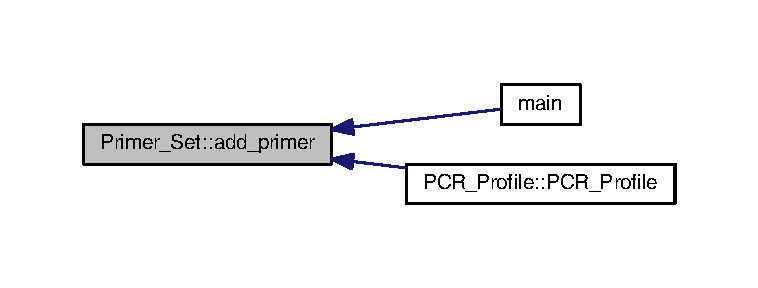
\includegraphics[width=350pt]{class_primer___set_a136e11664762cb801c833209a68204fe_icgraph}
\end{center}
\end{figure}
\mbox{\Hypertarget{class_primer___set_acbbf2f8583751542a18f895e44643be2}\label{class_primer___set_acbbf2f8583751542a18f895e44643be2}} 
\index{Primer\+\_\+\+Set@{Primer\+\_\+\+Set}!add\+\_\+primer@{add\+\_\+primer}}
\index{add\+\_\+primer@{add\+\_\+primer}!Primer\+\_\+\+Set@{Primer\+\_\+\+Set}}
\subsubsection{\texorpdfstring{add\+\_\+primer()}{add\_primer()}\hspace{0.1cm}{\footnotesize\ttfamily [2/2]}}
{\footnotesize\ttfamily bool Primer\+\_\+\+Set\+::add\+\_\+primer (\begin{DoxyParamCaption}\item[{char $\ast$}]{primer,  }\item[{ostream \&}]{err\+\_\+msg = {\ttfamily cout} }\end{DoxyParamCaption})}



Definition at line 288 of file Primer\+\_\+\+Set.\+h.

\mbox{\Hypertarget{class_primer___set_af45de3f0a9a7cac592aa66e15f1d6155}\label{class_primer___set_af45de3f0a9a7cac592aa66e15f1d6155}} 
\index{Primer\+\_\+\+Set@{Primer\+\_\+\+Set}!convert\+\_\+primer\+\_\+int\+\_\+to\+\_\+txt@{convert\+\_\+primer\+\_\+int\+\_\+to\+\_\+txt}}
\index{convert\+\_\+primer\+\_\+int\+\_\+to\+\_\+txt@{convert\+\_\+primer\+\_\+int\+\_\+to\+\_\+txt}!Primer\+\_\+\+Set@{Primer\+\_\+\+Set}}
\subsubsection{\texorpdfstring{convert\+\_\+primer\+\_\+int\+\_\+to\+\_\+txt()}{convert\_primer\_int\_to\_txt()}}
{\footnotesize\ttfamily bool Primer\+\_\+\+Set\+::convert\+\_\+primer\+\_\+int\+\_\+to\+\_\+txt (\begin{DoxyParamCaption}\item[{unsigned int}]{primer\+\_\+value,  }\item[{char $\ast$\&}]{primer,  }\item[{ostream \&}]{err\+\_\+msg = {\ttfamily cout} }\end{DoxyParamCaption})}



Definition at line 206 of file Primer\+\_\+\+Set.\+h.

\mbox{\Hypertarget{class_primer___set_a6f351e7eb9dc3ceb42beb4fcd368e616}\label{class_primer___set_a6f351e7eb9dc3ceb42beb4fcd368e616}} 
\index{Primer\+\_\+\+Set@{Primer\+\_\+\+Set}!convert\+\_\+primer\+\_\+to\+\_\+reverse\+\_\+complement@{convert\+\_\+primer\+\_\+to\+\_\+reverse\+\_\+complement}}
\index{convert\+\_\+primer\+\_\+to\+\_\+reverse\+\_\+complement@{convert\+\_\+primer\+\_\+to\+\_\+reverse\+\_\+complement}!Primer\+\_\+\+Set@{Primer\+\_\+\+Set}}
\subsubsection{\texorpdfstring{convert\+\_\+primer\+\_\+to\+\_\+reverse\+\_\+complement()}{convert\_primer\_to\_reverse\_complement()}}
{\footnotesize\ttfamily unsigned int Primer\+\_\+\+Set\+::convert\+\_\+primer\+\_\+to\+\_\+reverse\+\_\+complement (\begin{DoxyParamCaption}\item[{int}]{position,  }\item[{ostream \&}]{err\+\_\+msg = {\ttfamily cout} }\end{DoxyParamCaption})}



Definition at line 226 of file Primer\+\_\+\+Set.\+h.

\mbox{\Hypertarget{class_primer___set_a0691f55ba1bb6e1dca8fcd5cdfd6bd1a}\label{class_primer___set_a0691f55ba1bb6e1dca8fcd5cdfd6bd1a}} 
\index{Primer\+\_\+\+Set@{Primer\+\_\+\+Set}!convert\+\_\+primer\+\_\+txt\+\_\+to\+\_\+int@{convert\+\_\+primer\+\_\+txt\+\_\+to\+\_\+int}}
\index{convert\+\_\+primer\+\_\+txt\+\_\+to\+\_\+int@{convert\+\_\+primer\+\_\+txt\+\_\+to\+\_\+int}!Primer\+\_\+\+Set@{Primer\+\_\+\+Set}}
\subsubsection{\texorpdfstring{convert\+\_\+primer\+\_\+txt\+\_\+to\+\_\+int()}{convert\_primer\_txt\_to\_int()}}
{\footnotesize\ttfamily bool Primer\+\_\+\+Set\+::convert\+\_\+primer\+\_\+txt\+\_\+to\+\_\+int (\begin{DoxyParamCaption}\item[{char $\ast$}]{primer,  }\item[{unsigned int \&}]{primer\+\_\+value,  }\item[{ostream \&}]{err\+\_\+msg = {\ttfamily cout} }\end{DoxyParamCaption})}



Definition at line 86 of file Primer\+\_\+\+Set.\+h.

\mbox{\Hypertarget{class_primer___set_a1285be11e09dff32a28e8c36d01175c5}\label{class_primer___set_a1285be11e09dff32a28e8c36d01175c5}} 
\index{Primer\+\_\+\+Set@{Primer\+\_\+\+Set}!delete\+\_\+primer@{delete\+\_\+primer}}
\index{delete\+\_\+primer@{delete\+\_\+primer}!Primer\+\_\+\+Set@{Primer\+\_\+\+Set}}
\subsubsection{\texorpdfstring{delete\+\_\+primer()}{delete\_primer()}}
{\footnotesize\ttfamily bool Primer\+\_\+\+Set\+::delete\+\_\+primer (\begin{DoxyParamCaption}\item[{int $\ast$}]{position,  }\item[{unsigned int}]{number\+\_\+of\+\_\+primers\+\_\+to\+\_\+delete,  }\item[{ostream \&}]{err\+\_\+msg = {\ttfamily cout} }\end{DoxyParamCaption})}



Definition at line 295 of file Primer\+\_\+\+Set.\+h.

\mbox{\Hypertarget{class_primer___set_af9cc2185ff8cb758f383481d138faf8f}\label{class_primer___set_af9cc2185ff8cb758f383481d138faf8f}} 
\index{Primer\+\_\+\+Set@{Primer\+\_\+\+Set}!get\+\_\+number\+\_\+of\+\_\+primers@{get\+\_\+number\+\_\+of\+\_\+primers}}
\index{get\+\_\+number\+\_\+of\+\_\+primers@{get\+\_\+number\+\_\+of\+\_\+primers}!Primer\+\_\+\+Set@{Primer\+\_\+\+Set}}
\subsubsection{\texorpdfstring{get\+\_\+number\+\_\+of\+\_\+primers()}{get\_number\_of\_primers()}}
{\footnotesize\ttfamily unsigned int Primer\+\_\+\+Set\+::get\+\_\+number\+\_\+of\+\_\+primers (\begin{DoxyParamCaption}{ }\end{DoxyParamCaption})\hspace{0.3cm}{\ttfamily [inline]}}



Definition at line 57 of file Primer\+\_\+\+Set.\+h.

Here is the caller graph for this function\+:
\nopagebreak
\begin{figure}[H]
\begin{center}
\leavevmode
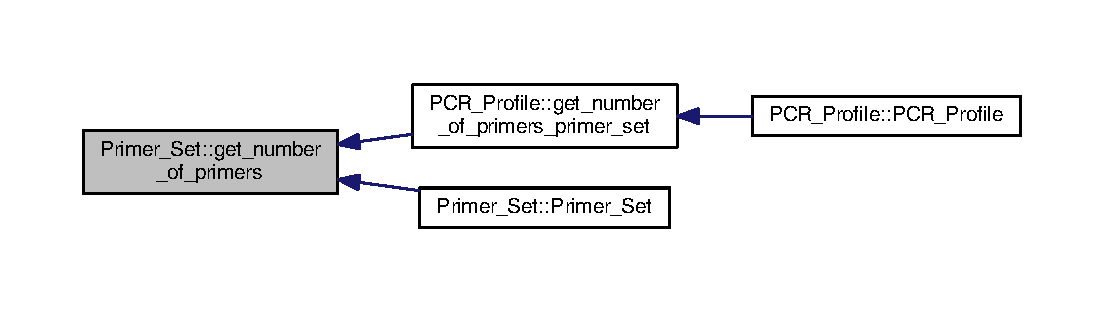
\includegraphics[width=350pt]{class_primer___set_af9cc2185ff8cb758f383481d138faf8f_icgraph}
\end{center}
\end{figure}
\mbox{\Hypertarget{class_primer___set_a4eae0937a142b6399cf5b4022f8897df}\label{class_primer___set_a4eae0937a142b6399cf5b4022f8897df}} 
\index{Primer\+\_\+\+Set@{Primer\+\_\+\+Set}!get\+\_\+pointer\+\_\+to\+\_\+primer\+\_\+array@{get\+\_\+pointer\+\_\+to\+\_\+primer\+\_\+array}}
\index{get\+\_\+pointer\+\_\+to\+\_\+primer\+\_\+array@{get\+\_\+pointer\+\_\+to\+\_\+primer\+\_\+array}!Primer\+\_\+\+Set@{Primer\+\_\+\+Set}}
\subsubsection{\texorpdfstring{get\+\_\+pointer\+\_\+to\+\_\+primer\+\_\+array()}{get\_pointer\_to\_primer\_array()}}
{\footnotesize\ttfamily unsigned int$\ast$ Primer\+\_\+\+Set\+::get\+\_\+pointer\+\_\+to\+\_\+primer\+\_\+array (\begin{DoxyParamCaption}{ }\end{DoxyParamCaption})\hspace{0.3cm}{\ttfamily [inline]}}



Definition at line 54 of file Primer\+\_\+\+Set.\+h.

\mbox{\Hypertarget{class_primer___set_ae795b4d40b4da9856b467f09462769e1}\label{class_primer___set_ae795b4d40b4da9856b467f09462769e1}} 
\index{Primer\+\_\+\+Set@{Primer\+\_\+\+Set}!get\+\_\+pointer\+\_\+to\+\_\+reverse\+\_\+complement\+\_\+primer\+\_\+array@{get\+\_\+pointer\+\_\+to\+\_\+reverse\+\_\+complement\+\_\+primer\+\_\+array}}
\index{get\+\_\+pointer\+\_\+to\+\_\+reverse\+\_\+complement\+\_\+primer\+\_\+array@{get\+\_\+pointer\+\_\+to\+\_\+reverse\+\_\+complement\+\_\+primer\+\_\+array}!Primer\+\_\+\+Set@{Primer\+\_\+\+Set}}
\subsubsection{\texorpdfstring{get\+\_\+pointer\+\_\+to\+\_\+reverse\+\_\+complement\+\_\+primer\+\_\+array()}{get\_pointer\_to\_reverse\_complement\_primer\_array()}}
{\footnotesize\ttfamily unsigned int$\ast$ Primer\+\_\+\+Set\+::get\+\_\+pointer\+\_\+to\+\_\+reverse\+\_\+complement\+\_\+primer\+\_\+array (\begin{DoxyParamCaption}{ }\end{DoxyParamCaption})\hspace{0.3cm}{\ttfamily [inline]}}



Definition at line 55 of file Primer\+\_\+\+Set.\+h.

\mbox{\Hypertarget{class_primer___set_a7c639e643b36dea739026862f12a64d4}\label{class_primer___set_a7c639e643b36dea739026862f12a64d4}} 
\index{Primer\+\_\+\+Set@{Primer\+\_\+\+Set}!get\+\_\+primer\+\_\+as\+\_\+value@{get\+\_\+primer\+\_\+as\+\_\+value}}
\index{get\+\_\+primer\+\_\+as\+\_\+value@{get\+\_\+primer\+\_\+as\+\_\+value}!Primer\+\_\+\+Set@{Primer\+\_\+\+Set}}
\subsubsection{\texorpdfstring{get\+\_\+primer\+\_\+as\+\_\+value()}{get\_primer\_as\_value()}}
{\footnotesize\ttfamily unsigned int Primer\+\_\+\+Set\+::get\+\_\+primer\+\_\+as\+\_\+value (\begin{DoxyParamCaption}\item[{unsigned int}]{position }\end{DoxyParamCaption})\hspace{0.3cm}{\ttfamily [inline]}}



Definition at line 40 of file Primer\+\_\+\+Set.\+h.

Here is the caller graph for this function\+:
\nopagebreak
\begin{figure}[H]
\begin{center}
\leavevmode
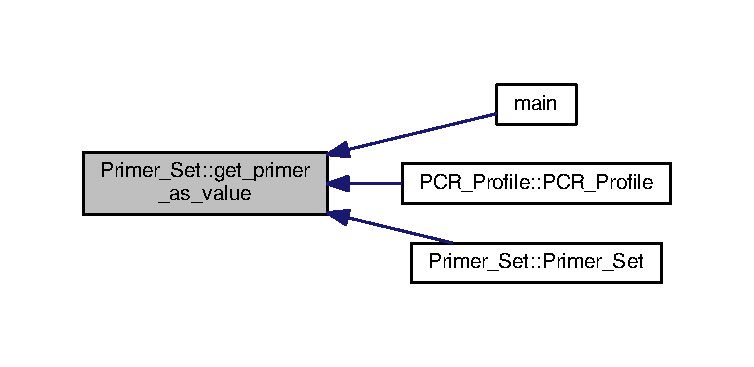
\includegraphics[width=350pt]{class_primer___set_a7c639e643b36dea739026862f12a64d4_icgraph}
\end{center}
\end{figure}
\mbox{\Hypertarget{class_primer___set_af53fe2ae85933f04a5cc2e159a3ed49f}\label{class_primer___set_af53fe2ae85933f04a5cc2e159a3ed49f}} 
\index{Primer\+\_\+\+Set@{Primer\+\_\+\+Set}!get\+\_\+primer\+\_\+length@{get\+\_\+primer\+\_\+length}}
\index{get\+\_\+primer\+\_\+length@{get\+\_\+primer\+\_\+length}!Primer\+\_\+\+Set@{Primer\+\_\+\+Set}}
\subsubsection{\texorpdfstring{get\+\_\+primer\+\_\+length()}{get\_primer\_length()}}
{\footnotesize\ttfamily unsigned int Primer\+\_\+\+Set\+::get\+\_\+primer\+\_\+length (\begin{DoxyParamCaption}{ }\end{DoxyParamCaption})\hspace{0.3cm}{\ttfamily [inline]}}



Definition at line 58 of file Primer\+\_\+\+Set.\+h.

Here is the caller graph for this function\+:
\nopagebreak
\begin{figure}[H]
\begin{center}
\leavevmode
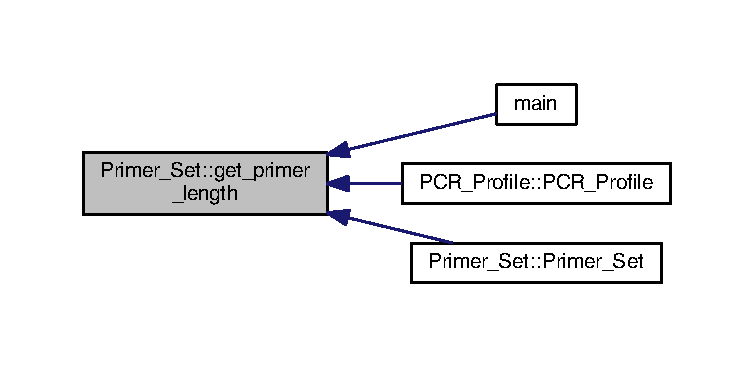
\includegraphics[width=350pt]{class_primer___set_af53fe2ae85933f04a5cc2e159a3ed49f_icgraph}
\end{center}
\end{figure}
\mbox{\Hypertarget{class_primer___set_aca0009d54b4b99a0a45d4e4995bb9818}\label{class_primer___set_aca0009d54b4b99a0a45d4e4995bb9818}} 
\index{Primer\+\_\+\+Set@{Primer\+\_\+\+Set}!show\+\_\+\+All@{show\+\_\+\+All}}
\index{show\+\_\+\+All@{show\+\_\+\+All}!Primer\+\_\+\+Set@{Primer\+\_\+\+Set}}
\subsubsection{\texorpdfstring{show\+\_\+\+All()}{show\_All()}}
{\footnotesize\ttfamily bool Primer\+\_\+\+Set\+::show\+\_\+\+All (\begin{DoxyParamCaption}\item[{ostream \&}]{out = {\ttfamily cout},  }\item[{ostream \&}]{err\+\_\+msg = {\ttfamily cout} }\end{DoxyParamCaption})}



Definition at line 247 of file Primer\+\_\+\+Set.\+h.

\mbox{\Hypertarget{class_primer___set_a86da618d3bafd760ceb21099b168e54c}\label{class_primer___set_a86da618d3bafd760ceb21099b168e54c}} 
\index{Primer\+\_\+\+Set@{Primer\+\_\+\+Set}!show\+\_\+statistics@{show\+\_\+statistics}}
\index{show\+\_\+statistics@{show\+\_\+statistics}!Primer\+\_\+\+Set@{Primer\+\_\+\+Set}}
\subsubsection{\texorpdfstring{show\+\_\+statistics()}{show\_statistics()}}
{\footnotesize\ttfamily bool Primer\+\_\+\+Set\+::show\+\_\+statistics (\begin{DoxyParamCaption}\item[{ostream \&}]{out = {\ttfamily cout},  }\item[{ostream \&}]{err\+\_\+msg = {\ttfamily cout} }\end{DoxyParamCaption})}



Definition at line 160 of file Primer\+\_\+\+Set.\+h.

\mbox{\Hypertarget{class_primer___set_a55d08f895a8af207b7e06abf8bf95f99}\label{class_primer___set_a55d08f895a8af207b7e06abf8bf95f99}} 
\index{Primer\+\_\+\+Set@{Primer\+\_\+\+Set}!write\+\_\+to\+\_\+file@{write\+\_\+to\+\_\+file}}
\index{write\+\_\+to\+\_\+file@{write\+\_\+to\+\_\+file}!Primer\+\_\+\+Set@{Primer\+\_\+\+Set}}
\subsubsection{\texorpdfstring{write\+\_\+to\+\_\+file()}{write\_to\_file()}}
{\footnotesize\ttfamily bool Primer\+\_\+\+Set\+::write\+\_\+to\+\_\+file (\begin{DoxyParamCaption}\item[{char $\ast$}]{filename,  }\item[{ostream \&}]{err\+\_\+msg = {\ttfamily cout} }\end{DoxyParamCaption})}



Definition at line 131 of file Primer\+\_\+\+Set.\+h.



The documentation for this class was generated from the following file\+:\begin{DoxyCompactItemize}
\item 
R\+P\+A/\mbox{\hyperlink{_primer___set_8h}{Primer\+\_\+\+Set.\+h}}\end{DoxyCompactItemize}

\hypertarget{class_sequence}{}\section{Sequence Class Reference}
\label{class_sequence}\index{Sequence@{Sequence}}
\subsection*{Public Member Functions}
\begin{DoxyCompactItemize}
\item 
\mbox{\Hypertarget{class_sequence_acdd11b606b266e81cc5b957e86b45517}\label{class_sequence_acdd11b606b266e81cc5b957e86b45517}} 
{\bfseries Sequence} (char $\ast$sequence, unsigned int sequence\+\_\+length, unsigned int primer\+\_\+length=0, ostream \&err\+\_\+msg=cout)
\item 
\mbox{\Hypertarget{class_sequence_ad6f16ee0cacbb22596c7a34d8a2f4c14}\label{class_sequence_ad6f16ee0cacbb22596c7a34d8a2f4c14}} 
{\bfseries Sequence} (\mbox{\hyperlink{class_sequence}{Sequence}} $\ast$\+\_\+sequence, unsigned int primer\+\_\+length=0, ostream \&err\+\_\+msg=cout)
\item 
\mbox{\Hypertarget{class_sequence_adfd0c2b8558f68f764a7690ed9ad4adc}\label{class_sequence_adfd0c2b8558f68f764a7690ed9ad4adc}} 
bool {\bfseries show\+\_\+statistics} (ostream \&out=cout, ostream \&err\+\_\+msg=cout)
\item 
\mbox{\Hypertarget{class_sequence_a01816c20cdd1c716a30b03c24a5a2b7f}\label{class_sequence_a01816c20cdd1c716a30b03c24a5a2b7f}} 
bool {\bfseries show\+\_\+\+All} (ostream \&out=cout, ostream \&err\+\_\+msg=cout)
\item 
\mbox{\Hypertarget{class_sequence_a9c1e7770390e4f1d02ae250d640a32a7}\label{class_sequence_a9c1e7770390e4f1d02ae250d640a32a7}} 
char $\ast$ {\bfseries get\+\_\+pointer\+\_\+to\+\_\+sequence} ()
\item 
\mbox{\Hypertarget{class_sequence_af37c4ac41b89a5081ca71ff2a9d9bd1c}\label{class_sequence_af37c4ac41b89a5081ca71ff2a9d9bd1c}} 
unsigned int $\ast$ {\bfseries get\+\_\+pointer\+\_\+to\+\_\+sequence\+\_\+int} ()
\item 
\mbox{\Hypertarget{class_sequence_a5454c394570fa19c2b0ac771c6e74097}\label{class_sequence_a5454c394570fa19c2b0ac771c6e74097}} 
int {\bfseries get\+\_\+sequence\+\_\+length} ()
\end{DoxyCompactItemize}


The documentation for this class was generated from the following file\+:\begin{DoxyCompactItemize}
\item 
C\+:/\+Users/\+Kamil/\+Documents/\+R\+P\+A-\/\+Optimization/\+R\+P\+A/Sequence.\+h\end{DoxyCompactItemize}

\hypertarget{struct_sortable___pareto}{}\section{Sortable\+\_\+\+Pareto Struct Reference}
\label{struct_sortable___pareto}\index{Sortable\+\_\+\+Pareto@{Sortable\+\_\+\+Pareto}}
\subsection*{Public Attributes}
\begin{DoxyCompactItemize}
\item 
\mbox{\Hypertarget{struct_sortable___pareto_ad86fc6339ac5d0a90214bcfe29f2d878}\label{struct_sortable___pareto_ad86fc6339ac5d0a90214bcfe29f2d878}} 
unsigned int {\bfseries index}
\item 
\mbox{\Hypertarget{struct_sortable___pareto_ae5c3b332c8a192961de0a085d59432da}\label{struct_sortable___pareto_ae5c3b332c8a192961de0a085d59432da}} 
double {\bfseries x}
\item 
\mbox{\Hypertarget{struct_sortable___pareto_a00f29310c191ed10f9a6b58977be1bd7}\label{struct_sortable___pareto_a00f29310c191ed10f9a6b58977be1bd7}} 
double {\bfseries y}
\item 
\mbox{\Hypertarget{struct_sortable___pareto_a0e2e26ce019397c46470e63af05fc5c7}\label{struct_sortable___pareto_a0e2e26ce019397c46470e63af05fc5c7}} 
bool {\bfseries pareto\+\_\+set}
\end{DoxyCompactItemize}


The documentation for this struct was generated from the following file\+:\begin{DoxyCompactItemize}
\item 
C\+:/\+Users/\+Kamil/\+Documents/\+R\+P\+A-\/\+Optimization/\+R\+P\+A/Optimization\+\_\+\+Toolbox.\+h\end{DoxyCompactItemize}

%--- End generated contents ---

% Index
\backmatter
\newpage
\phantomsection
\clearemptydoublepage
\addcontentsline{toc}{chapter}{Index}
\printindex

\end{document}
